\documentclass[twoside]{book}

% Packages required by doxygen
\usepackage{calc}
\usepackage{doxygen}
\usepackage{graphicx}
\usepackage[utf8]{inputenc}
\usepackage{makeidx}
\usepackage{multicol}
\usepackage{multirow}
\usepackage{textcomp}
\usepackage[table]{xcolor}

% Font selection
\usepackage[T1]{fontenc}
\usepackage{mathptmx}
\usepackage[scaled=.90]{helvet}
\usepackage{courier}
\usepackage{amssymb}
\usepackage{sectsty}
\renewcommand{\familydefault}{\sfdefault}
\allsectionsfont{%
  \fontseries{bc}\selectfont%
  \color{darkgray}%
}
\renewcommand{\DoxyLabelFont}{%
  \fontseries{bc}\selectfont%
  \color{darkgray}%
}

% Page & text layout
\usepackage{geometry}
\geometry{%
  a4paper,%
  top=2.5cm,%
  bottom=2.5cm,%
  left=2.5cm,%
  right=2.5cm%
}
\tolerance=750
\hfuzz=15pt
\hbadness=750
\setlength{\emergencystretch}{15pt}
\setlength{\parindent}{0cm}
\setlength{\parskip}{0.2cm}
\makeatletter
\renewcommand{\paragraph}{%
  \@startsection{paragraph}{4}{0ex}{-1.0ex}{1.0ex}{%
    \normalfont\normalsize\bfseries\SS@parafont%
  }%
}
\renewcommand{\subparagraph}{%
  \@startsection{subparagraph}{5}{0ex}{-1.0ex}{1.0ex}{%
    \normalfont\normalsize\bfseries\SS@subparafont%
  }%
}
\makeatother

% Headers & footers
\usepackage{fancyhdr}
\pagestyle{fancyplain}
\fancyhead[LE]{\fancyplain{}{\bfseries\thepage}}
\fancyhead[CE]{\fancyplain{}{}}
\fancyhead[RE]{\fancyplain{}{\bfseries\leftmark}}
\fancyhead[LO]{\fancyplain{}{\bfseries\rightmark}}
\fancyhead[CO]{\fancyplain{}{}}
\fancyhead[RO]{\fancyplain{}{\bfseries\thepage}}
\fancyfoot[LE]{\fancyplain{}{}}
\fancyfoot[CE]{\fancyplain{}{}}
\fancyfoot[RE]{\fancyplain{}{\bfseries\scriptsize Generated on Sat Jun 3 2017 18\-:24\-:59 for S\-Q\-Lite\-X\-X by Doxygen }}
\fancyfoot[LO]{\fancyplain{}{\bfseries\scriptsize Generated on Sat Jun 3 2017 18\-:24\-:59 for S\-Q\-Lite\-X\-X by Doxygen }}
\fancyfoot[CO]{\fancyplain{}{}}
\fancyfoot[RO]{\fancyplain{}{}}
\renewcommand{\footrulewidth}{0.4pt}
\renewcommand{\chaptermark}[1]{%
  \markboth{#1}{}%
}
\renewcommand{\sectionmark}[1]{%
  \markright{\thesection\ #1}%
}

% Indices & bibliography
\usepackage{natbib}
\usepackage[titles]{tocloft}
\setcounter{tocdepth}{3}
\setcounter{secnumdepth}{5}
\makeindex

% Hyperlinks (required, but should be loaded last)
\usepackage{ifpdf}
\ifpdf
  \usepackage[pdftex,pagebackref=true]{hyperref}
\else
  \usepackage[ps2pdf,pagebackref=true]{hyperref}
\fi
\hypersetup{%
  colorlinks=true,%
  linkcolor=blue,%
  citecolor=blue,%
  unicode%
}

% Custom commands
\newcommand{\clearemptydoublepage}{%
  \newpage{\pagestyle{empty}\cleardoublepage}%
}


%===== C O N T E N T S =====

\begin{document}

% Titlepage & ToC
\hypersetup{pageanchor=false}
\pagenumbering{roman}
\begin{titlepage}
\vspace*{7cm}
\begin{center}%
{\Large S\-Q\-Lite\-X\-X \\[1ex]\large .. }\\
\vspace*{1cm}
{\large Generated by Doxygen 1.8.6}\\
\vspace*{0.5cm}
{\small Sat Jun 3 2017 18:24:59}\\
\end{center}
\end{titlepage}
\clearemptydoublepage
\tableofcontents
\clearemptydoublepage
\pagenumbering{arabic}
\hypersetup{pageanchor=true}

%--- Begin generated contents ---
\chapter{Hierarchical Index}
\section{Class Hierarchy}
This inheritance list is sorted roughly, but not completely, alphabetically\-:\begin{DoxyCompactList}
\item \contentsline{section}{sqlite\-:\-:backup}{\pageref{a00001}}{}
\item \contentsline{section}{sqlite\-:\-:blob}{\pageref{a00002}}{}
\item \contentsline{section}{sqlite\-:\-:dbconnection}{\pageref{a00004}}{}
\item \contentsline{section}{sqlite\-:\-:exception}{\pageref{a00006}}{}
\begin{DoxyCompactList}
\item \contentsline{section}{sqlite\-:\-:busy\-\_\-exception}{\pageref{a00003}}{}
\end{DoxyCompactList}
\item \contentsline{section}{sqlite\-:\-:mutex}{\pageref{a00009}}{}
\item \contentsline{section}{sqlite\-:\-:reader$<$ T $>$}{\pageref{a00010}}{}
\item \contentsline{section}{sqlite\-:\-:reader$<$ row $>$}{\pageref{a00010}}{}
\begin{DoxyCompactList}
\item \contentsline{section}{sqlite\-:\-:row}{\pageref{a00011}}{}
\end{DoxyCompactList}
\item \contentsline{section}{sqlite\-:\-:reader$<$ statement $>$}{\pageref{a00010}}{}
\begin{DoxyCompactList}
\item \contentsline{section}{sqlite\-:\-:statement}{\pageref{a00013}}{}
\end{DoxyCompactList}
\item \contentsline{section}{sqlite\-:\-:row\-\_\-iterator}{\pageref{a00012}}{}
\item \contentsline{section}{sqlite\-:\-:transaction}{\pageref{a00014}}{}
\begin{DoxyCompactList}
\item \contentsline{section}{sqlite\-:\-:deferred\-\_\-transaction}{\pageref{a00005}}{}
\item \contentsline{section}{sqlite\-:\-:exclusive\-\_\-transaction}{\pageref{a00007}}{}
\item \contentsline{section}{sqlite\-:\-:immediate\-\_\-transaction}{\pageref{a00008}}{}
\end{DoxyCompactList}
\item \contentsline{section}{sqlite\-:\-:value}{\pageref{a00015}}{}
\end{DoxyCompactList}

\chapter{Class Index}
\section{Class List}
Here are the classes, structs, unions and interfaces with brief descriptions\-:\begin{DoxyCompactList}
\item\contentsline{section}{\hyperlink{a00001}{sqlite\-::backup} \\*Used to aid in the process of backing up a database }{\pageref{a00001}}{}
\item\contentsline{section}{\hyperlink{a00002}{sqlite\-::blob} \\*A \char`\"{}\-Binary Large O\-Bject\char`\"{} }{\pageref{a00002}}{}
\item\contentsline{section}{\hyperlink{a00003}{sqlite\-::busy\-\_\-exception} \\*Encapsulation of the S\-Q\-L\-I\-T\-E\-\_\-\-B\-U\-S\-Y error code derived from S\-Q\-Lite\-::\-Exception }{\pageref{a00003}}{}
\item\contentsline{section}{\hyperlink{a00004}{sqlite\-::dbconnection} \\*Class that represents a connection to a database }{\pageref{a00004}}{}
\item\contentsline{section}{\hyperlink{a00005}{sqlite\-::deferred\-\_\-transaction} \\*R\-A\-I\-I encapsulation of the \hyperlink{a00038}{S\-Q\-Lite} deferred transaction }{\pageref{a00005}}{}
\item\contentsline{section}{\hyperlink{a00006}{sqlite\-::exception} \\*Encapsulation of the error code and message from S\-Q\-Lite3, based on std\-::runtime\-\_\-error }{\pageref{a00006}}{}
\item\contentsline{section}{\hyperlink{a00007}{sqlite\-::exclusive\-\_\-transaction} \\*R\-A\-I\-I encapsulation of the \hyperlink{a00038}{S\-Q\-Lite} exclusive transaction }{\pageref{a00007}}{}
\item\contentsline{section}{\hyperlink{a00008}{sqlite\-::immediate\-\_\-transaction} \\*R\-A\-I\-I encapsulation of the \hyperlink{a00038}{S\-Q\-Lite} immediate transaction }{\pageref{a00008}}{}
\item\contentsline{section}{\hyperlink{a00009}{sqlite\-::mutex} \\*Helps with serializing access to a database connection }{\pageref{a00009}}{}
\item\contentsline{section}{\hyperlink{a00010}{sqlite\-::reader$<$ T $>$} \\*Base class used to help with reading \char`\"{}sqlite3\-\_\-stmt\char`\"{} information }{\pageref{a00010}}{}
\item\contentsline{section}{\hyperlink{a00011}{sqlite\-::row} \\*Represents a returned row when stepping through a \char`\"{}\-S\-E\-L\-E\-C\-T\char`\"{} statement }{\pageref{a00011}}{}
\item\contentsline{section}{\hyperlink{a00012}{sqlite\-::row\-\_\-iterator} \\*Helps when iterating over rows in a \char`\"{}\-S\-E\-L\-E\-C\-T\char`\"{} statement }{\pageref{a00012}}{}
\item\contentsline{section}{\hyperlink{a00013}{sqlite\-::statement} \\*Represents a single S\-Q\-L statement that has been compiled into binary form and is ready to be evaluated, aka \char`\"{}sqlite3\-\_\-stmt\char`\"{} }{\pageref{a00013}}{}
\item\contentsline{section}{\hyperlink{a00014}{sqlite\-::transaction} \\*R\-A\-I\-I encapsulation of the \hyperlink{a00038}{S\-Q\-Lite} Transactions }{\pageref{a00014}}{}
\item\contentsline{section}{\hyperlink{a00015}{sqlite\-::value} \\*A \hyperlink{a00038}{S\-Q\-Lite} dynamically typed value object, aka \char`\"{}sqlite3\-\_\-value\char`\"{} }{\pageref{a00015}}{}
\end{DoxyCompactList}

\chapter{Class Documentation}
\hypertarget{class_s_q_lite_1_1aggregate__wrapper}{\section{S\-Q\-Lite\-:\-:aggregate\-\_\-wrapper$<$ T $>$ Class Template Reference}
\label{class_s_q_lite_1_1aggregate__wrapper}\index{S\-Q\-Lite\-::aggregate\-\_\-wrapper$<$ T $>$@{S\-Q\-Lite\-::aggregate\-\_\-wrapper$<$ T $>$}}
}
\subsection*{Public Member Functions}
\begin{DoxyCompactItemize}
\item 
\hypertarget{class_s_q_lite_1_1aggregate__wrapper_afa2234420d5123fb9c2f32cdeb141d5c}{void {\bfseries step} (sqlite3\-\_\-context $\ast$context, int argc, sqlite3\-\_\-value $\ast$$\ast$values)}\label{class_s_q_lite_1_1aggregate__wrapper_afa2234420d5123fb9c2f32cdeb141d5c}

\item 
\hypertarget{class_s_q_lite_1_1aggregate__wrapper_a81833a66bb5aff5c6a6721c5d4e922ab}{void {\bfseries finalize} (sqlite3\-\_\-context $\ast$context)}\label{class_s_q_lite_1_1aggregate__wrapper_a81833a66bb5aff5c6a6721c5d4e922ab}

\item 
\hypertarget{class_s_q_lite_1_1aggregate__wrapper_a42dfb0198b091c777f066ce1c4e04f2e}{void {\bfseries reset} ()}\label{class_s_q_lite_1_1aggregate__wrapper_a42dfb0198b091c777f066ce1c4e04f2e}

\end{DoxyCompactItemize}


The documentation for this class was generated from the following file\-:\begin{DoxyCompactItemize}
\item 
src/Functions.\-h\end{DoxyCompactItemize}

\hypertarget{struct_s_q_lite_1_1function__traits_3_01_r_07_c_1_1_5_08_07_args_8_8_8_08_4_1_1arg}{\section{S\-Q\-Lite\-:\-:function\-\_\-traits$<$ R(C\-:\-:$\ast$)(Args...)$>$\-:\-:arg$<$ i $>$ Struct Template Reference}
\label{struct_s_q_lite_1_1function__traits_3_01_r_07_c_1_1_5_08_07_args_8_8_8_08_4_1_1arg}\index{S\-Q\-Lite\-::function\-\_\-traits$<$ R(\-C\-::$\ast$)(\-Args...)$>$\-::arg$<$ i $>$@{S\-Q\-Lite\-::function\-\_\-traits$<$ R(\-C\-::$\ast$)(\-Args...)$>$\-::arg$<$ i $>$}}
}
\subsection*{Public Types}
\begin{DoxyCompactItemize}
\item 
\hypertarget{struct_s_q_lite_1_1function__traits_3_01_r_07_c_1_1_5_08_07_args_8_8_8_08_4_1_1arg_a514126a7a2361abdb9edcf202428c8b4}{typedef std\-::tuple\-\_\-element$<$ i, \\*
std\-::tuple$<$ Args...$>$ $>$\-::type {\bfseries type}}\label{struct_s_q_lite_1_1function__traits_3_01_r_07_c_1_1_5_08_07_args_8_8_8_08_4_1_1arg_a514126a7a2361abdb9edcf202428c8b4}

\end{DoxyCompactItemize}


The documentation for this struct was generated from the following file\-:\begin{DoxyCompactItemize}
\item 
src/Functions.\-h\end{DoxyCompactItemize}

\hypertarget{struct_s_q_lite_1_1function__traits_3_01_r_07_6_08_07_args_8_8_8_08_4_1_1arg}{\section{S\-Q\-Lite\-:\-:function\-\_\-traits$<$ R(\&)(Args...)$>$\-:\-:arg$<$ i $>$ Struct Template Reference}
\label{struct_s_q_lite_1_1function__traits_3_01_r_07_6_08_07_args_8_8_8_08_4_1_1arg}\index{S\-Q\-Lite\-::function\-\_\-traits$<$ R(\&)(\-Args...)$>$\-::arg$<$ i $>$@{S\-Q\-Lite\-::function\-\_\-traits$<$ R(\&)(\-Args...)$>$\-::arg$<$ i $>$}}
}
\subsection*{Public Types}
\begin{DoxyCompactItemize}
\item 
\hypertarget{struct_s_q_lite_1_1function__traits_3_01_r_07_6_08_07_args_8_8_8_08_4_1_1arg_aa2ed486a23fd9ee59fd508ea5f5fdfb7}{typedef std\-::tuple\-\_\-element$<$ i, \\*
std\-::tuple$<$ Args...$>$ $>$\-::type {\bfseries type}}\label{struct_s_q_lite_1_1function__traits_3_01_r_07_6_08_07_args_8_8_8_08_4_1_1arg_aa2ed486a23fd9ee59fd508ea5f5fdfb7}

\end{DoxyCompactItemize}


The documentation for this struct was generated from the following file\-:\begin{DoxyCompactItemize}
\item 
src/Functions.\-h\end{DoxyCompactItemize}

\hypertarget{struct_s_q_lite_1_1function__traits_3_01_r_07_c_1_1_5_08_07_args_8_8_8_08_01const_01_01_4_1_1arg}{\section{S\-Q\-Lite\-:\-:function\-\_\-traits$<$ R(C\-:\-:$\ast$)(Args...) const $>$\-:\-:arg$<$ i $>$ Struct Template Reference}
\label{struct_s_q_lite_1_1function__traits_3_01_r_07_c_1_1_5_08_07_args_8_8_8_08_01const_01_01_4_1_1arg}\index{S\-Q\-Lite\-::function\-\_\-traits$<$ R(\-C\-::$\ast$)(\-Args...) const  $>$\-::arg$<$ i $>$@{S\-Q\-Lite\-::function\-\_\-traits$<$ R(\-C\-::$\ast$)(\-Args...) const  $>$\-::arg$<$ i $>$}}
}
\subsection*{Public Types}
\begin{DoxyCompactItemize}
\item 
\hypertarget{struct_s_q_lite_1_1function__traits_3_01_r_07_c_1_1_5_08_07_args_8_8_8_08_01const_01_01_4_1_1arg_a7785567b43a6fb69906f09403f99e31f}{typedef std\-::tuple\-\_\-element$<$ i, \\*
std\-::tuple$<$ Args...$>$ $>$\-::type {\bfseries type}}\label{struct_s_q_lite_1_1function__traits_3_01_r_07_c_1_1_5_08_07_args_8_8_8_08_01const_01_01_4_1_1arg_a7785567b43a6fb69906f09403f99e31f}

\end{DoxyCompactItemize}


The documentation for this struct was generated from the following file\-:\begin{DoxyCompactItemize}
\item 
src/Functions.\-h\end{DoxyCompactItemize}

\hypertarget{struct_s_q_lite_1_1function__traits_3_01_r_07_5_08_07_args_8_8_8_08_4_1_1arg}{\section{S\-Q\-Lite\-:\-:function\-\_\-traits$<$ R($\ast$)(Args...)$>$\-:\-:arg$<$ i $>$ Struct Template Reference}
\label{struct_s_q_lite_1_1function__traits_3_01_r_07_5_08_07_args_8_8_8_08_4_1_1arg}\index{S\-Q\-Lite\-::function\-\_\-traits$<$ R($\ast$)(\-Args...)$>$\-::arg$<$ i $>$@{S\-Q\-Lite\-::function\-\_\-traits$<$ R($\ast$)(\-Args...)$>$\-::arg$<$ i $>$}}
}
\subsection*{Public Types}
\begin{DoxyCompactItemize}
\item 
\hypertarget{struct_s_q_lite_1_1function__traits_3_01_r_07_5_08_07_args_8_8_8_08_4_1_1arg_a4f793702bdbf828c51c2d891df8bb8ce}{typedef std\-::tuple\-\_\-element$<$ i, \\*
std\-::tuple$<$ Args...$>$ $>$\-::type {\bfseries type}}\label{struct_s_q_lite_1_1function__traits_3_01_r_07_5_08_07_args_8_8_8_08_4_1_1arg_a4f793702bdbf828c51c2d891df8bb8ce}

\end{DoxyCompactItemize}


The documentation for this struct was generated from the following file\-:\begin{DoxyCompactItemize}
\item 
src/Functions.\-h\end{DoxyCompactItemize}

\hypertarget{class_s_q_lite_1_1_backup}{\section{S\-Q\-Lite\-:\-:Backup Class Reference}
\label{class_s_q_lite_1_1_backup}\index{S\-Q\-Lite\-::\-Backup@{S\-Q\-Lite\-::\-Backup}}
}
\subsection*{Public Member Functions}
\begin{DoxyCompactItemize}
\item 
\hypertarget{class_s_q_lite_1_1_backup_a85bff6db538293ba839003bab73335c3}{{\bfseries Backup} (const \hyperlink{class_s_q_lite_1_1_backup}{Backup} \&other)=delete}\label{class_s_q_lite_1_1_backup_a85bff6db538293ba839003bab73335c3}

\item 
\hypertarget{class_s_q_lite_1_1_backup_abf35a70084311262e4121e7f7fe06fe8}{\hyperlink{class_s_q_lite_1_1_backup}{Backup} \& {\bfseries operator=} (\hyperlink{class_s_q_lite_1_1_backup}{Backup} \&other)=delete}\label{class_s_q_lite_1_1_backup_abf35a70084311262e4121e7f7fe06fe8}

\item 
\hypertarget{class_s_q_lite_1_1_backup_af2b065a181ac9ed81273d1360c4787bd}{{\bfseries Backup} (\hyperlink{class_s_q_lite_1_1_d_b_connection}{D\-B\-Connection} const \&source, \hyperlink{class_s_q_lite_1_1_d_b_connection}{D\-B\-Connection} const \&destination, const std\-::string \&source\-Name=\char`\"{}main\char`\"{}, const std\-::string \&destination\-Name=\char`\"{}main\char`\"{})}\label{class_s_q_lite_1_1_backup_af2b065a181ac9ed81273d1360c4787bd}

\item 
\hypertarget{class_s_q_lite_1_1_backup_a6ec2f5a0d8db598c15311437c4b9aa43}{bool {\bfseries step} (const int pages=-\/1)}\label{class_s_q_lite_1_1_backup_a6ec2f5a0d8db598c15311437c4b9aa43}

\item 
\hypertarget{class_s_q_lite_1_1_backup_aa4065df5ee53f85250b0204a28b2b9a9}{int {\bfseries get\-Total\-Page\-Count} ()}\label{class_s_q_lite_1_1_backup_aa4065df5ee53f85250b0204a28b2b9a9}

\item 
\hypertarget{class_s_q_lite_1_1_backup_a60ec7f043380c27b89c8b574e6360294}{int {\bfseries get\-Remaining\-Page\-Count} ()}\label{class_s_q_lite_1_1_backup_a60ec7f043380c27b89c8b574e6360294}

\item 
\hypertarget{class_s_q_lite_1_1_backup_ad2378b89c6ff3354a6852fea18c3c9f9}{sqlite3\-\_\-backup $\ast$ {\bfseries get\-Handle} () const noexcept}\label{class_s_q_lite_1_1_backup_ad2378b89c6ff3354a6852fea18c3c9f9}

\end{DoxyCompactItemize}


The documentation for this class was generated from the following files\-:\begin{DoxyCompactItemize}
\item 
src/Backup.\-h\item 
src/Backup.\-cpp\end{DoxyCompactItemize}

\hypertarget{class_s_q_lite_1_1_blob}{\section{S\-Q\-Lite\-:\-:Blob Class Reference}
\label{class_s_q_lite_1_1_blob}\index{S\-Q\-Lite\-::\-Blob@{S\-Q\-Lite\-::\-Blob}}
}
\subsection*{Public Member Functions}
\begin{DoxyCompactItemize}
\item 
\hypertarget{class_s_q_lite_1_1_blob_a9a12b838ed72118e90f41e256dc7d0ec}{{\bfseries Blob} (const void $\ast$data, int \hyperlink{class_s_q_lite_1_1_blob_a3a1316074209aeea955b8b1bf31e7a78}{size})}\label{class_s_q_lite_1_1_blob_a9a12b838ed72118e90f41e256dc7d0ec}

\item 
\hypertarget{class_s_q_lite_1_1_blob_a4f525d8e11e4361b808692eccb4e12a5}{{\bfseries Blob} (const \hyperlink{class_s_q_lite_1_1_blob}{Blob} \&other)}\label{class_s_q_lite_1_1_blob_a4f525d8e11e4361b808692eccb4e12a5}

\item 
\hypertarget{class_s_q_lite_1_1_blob_ae458297c2b9be504111c7b23636942e0}{{\bfseries Blob} (\hyperlink{class_s_q_lite_1_1_blob}{Blob} \&\&other)}\label{class_s_q_lite_1_1_blob_ae458297c2b9be504111c7b23636942e0}

\item 
\hypertarget{class_s_q_lite_1_1_blob_af34146d8ac8d1414c5ad1673ca05669e}{\hyperlink{class_s_q_lite_1_1_blob}{Blob} \& {\bfseries operator=} (const \hyperlink{class_s_q_lite_1_1_blob}{Blob} \&other)}\label{class_s_q_lite_1_1_blob_af34146d8ac8d1414c5ad1673ca05669e}

\item 
\hypertarget{class_s_q_lite_1_1_blob_ae6409ebce61480b97f01c072f9e49276}{\hyperlink{class_s_q_lite_1_1_blob}{Blob} \& {\bfseries operator=} (\hyperlink{class_s_q_lite_1_1_blob}{Blob} \&\&other)}\label{class_s_q_lite_1_1_blob_ae6409ebce61480b97f01c072f9e49276}

\item 
\hypertarget{class_s_q_lite_1_1_blob_a112b54351792991f10563295e33600e2}{const void $\ast$ {\bfseries data} () const }\label{class_s_q_lite_1_1_blob_a112b54351792991f10563295e33600e2}

\item 
int \hyperlink{class_s_q_lite_1_1_blob_a3a1316074209aeea955b8b1bf31e7a78}{size} () const 
\begin{DoxyCompactList}\small\item\em Used to get the size of the contained 'blob'. \end{DoxyCompactList}\end{DoxyCompactItemize}


\subsection{Member Function Documentation}
\hypertarget{class_s_q_lite_1_1_blob_a3a1316074209aeea955b8b1bf31e7a78}{\index{S\-Q\-Lite\-::\-Blob@{S\-Q\-Lite\-::\-Blob}!size@{size}}
\index{size@{size}!SQLite::Blob@{S\-Q\-Lite\-::\-Blob}}
\subsubsection[{size}]{\setlength{\rightskip}{0pt plus 5cm}int S\-Q\-Lite\-::\-Blob\-::size (
\begin{DoxyParamCaption}
{}
\end{DoxyParamCaption}
) const}}\label{class_s_q_lite_1_1_blob_a3a1316074209aeea955b8b1bf31e7a78}


Used to get the size of the contained 'blob'. 

\begin{DoxyReturn}{Returns}
the size in bytes of the contained 'blob' 
\end{DoxyReturn}


The documentation for this class was generated from the following files\-:\begin{DoxyCompactItemize}
\item 
src/Blob.\-h\item 
src/Blob.\-cpp\end{DoxyCompactItemize}

\hypertarget{class_s_q_lite_1_1_busy_exception}{\section{S\-Q\-Lite\-:\-:Busy\-Exception Class Reference}
\label{class_s_q_lite_1_1_busy_exception}\index{S\-Q\-Lite\-::\-Busy\-Exception@{S\-Q\-Lite\-::\-Busy\-Exception}}
}


Encapsulation of the S\-Q\-L\-I\-T\-E\-\_\-\-B\-U\-S\-Y error code derived from \hyperlink{class_s_q_lite_1_1_exception}{S\-Q\-Lite\-::\-Exception}.  




{\ttfamily \#include $<$Exception.\-h$>$}

Inheritance diagram for S\-Q\-Lite\-:\-:Busy\-Exception\-:\begin{figure}[H]
\begin{center}
\leavevmode
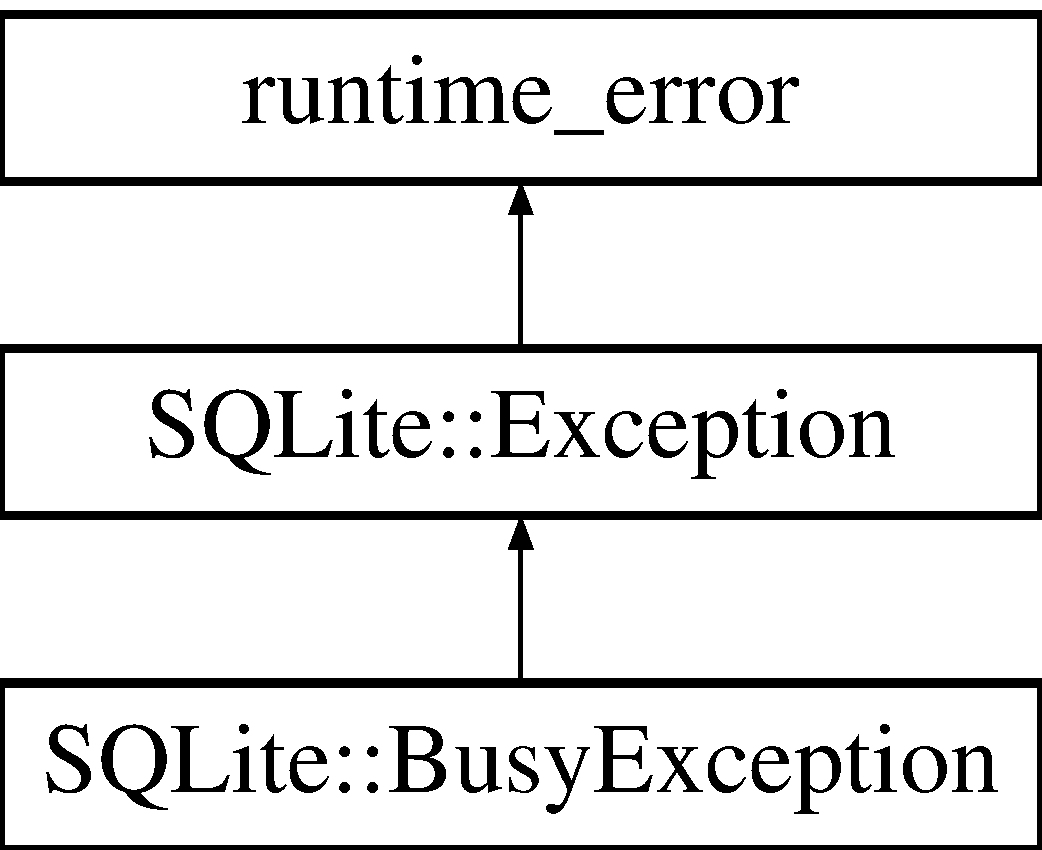
\includegraphics[height=3.000000cm]{class_s_q_lite_1_1_busy_exception}
\end{center}
\end{figure}
\subsection*{Public Member Functions}
\begin{DoxyCompactItemize}
\item 
\hypertarget{class_s_q_lite_1_1_busy_exception_ac6679ad9fcb996ce723941c7b590603e}{{\bfseries Busy\-Exception} (sqlite3 $\ast$const connection)}\label{class_s_q_lite_1_1_busy_exception_ac6679ad9fcb996ce723941c7b590603e}

\item 
\hypertarget{class_s_q_lite_1_1_busy_exception_aab5d5d7fd7dacb68eca8c9ceceb50619}{{\bfseries Busy\-Exception} (const std\-::string \&message)}\label{class_s_q_lite_1_1_busy_exception_aab5d5d7fd7dacb68eca8c9ceceb50619}

\end{DoxyCompactItemize}
\subsection*{Additional Inherited Members}


\subsection{Detailed Description}
Encapsulation of the S\-Q\-L\-I\-T\-E\-\_\-\-B\-U\-S\-Y error code derived from \hyperlink{class_s_q_lite_1_1_exception}{S\-Q\-Lite\-::\-Exception}. 



The documentation for this class was generated from the following file\-:\begin{DoxyCompactItemize}
\item 
src/Exception.\-h\end{DoxyCompactItemize}

\hypertarget{class_s_q_lite_1_1_d_b_connection}{\section{S\-Q\-Lite\-:\-:D\-B\-Connection Class Reference}
\label{class_s_q_lite_1_1_d_b_connection}\index{S\-Q\-Lite\-::\-D\-B\-Connection@{S\-Q\-Lite\-::\-D\-B\-Connection}}
}


Class that represents a connection to the database.  




{\ttfamily \#include $<$D\-B\-Connection.\-h$>$}

\subsection*{Public Member Functions}
\begin{DoxyCompactItemize}
\item 
\hypertarget{class_s_q_lite_1_1_d_b_connection_ab3dbee23694c323481260b84ff901403}{{\bfseries D\-B\-Connection} (const \hyperlink{class_s_q_lite_1_1_d_b_connection}{D\-B\-Connection} \&other) noexcept}\label{class_s_q_lite_1_1_d_b_connection_ab3dbee23694c323481260b84ff901403}

\item 
\hypertarget{class_s_q_lite_1_1_d_b_connection_a41cc922e68047f709c25283b9d0176d5}{{\bfseries D\-B\-Connection} (\hyperlink{class_s_q_lite_1_1_d_b_connection}{D\-B\-Connection} \&\&other) noexcept}\label{class_s_q_lite_1_1_d_b_connection_a41cc922e68047f709c25283b9d0176d5}

\item 
\hypertarget{class_s_q_lite_1_1_d_b_connection_abf18d7c37cf19fe46af7b6c7c0f0e8f2}{\hyperlink{class_s_q_lite_1_1_d_b_connection}{D\-B\-Connection} \& {\bfseries operator=} (const \hyperlink{class_s_q_lite_1_1_d_b_connection}{D\-B\-Connection} \&other) noexcept}\label{class_s_q_lite_1_1_d_b_connection_abf18d7c37cf19fe46af7b6c7c0f0e8f2}

\item 
\hypertarget{class_s_q_lite_1_1_d_b_connection_a2d10766ea45bfb79f4959e62d432feeb}{\hyperlink{class_s_q_lite_1_1_d_b_connection}{D\-B\-Connection} \& {\bfseries operator=} (\hyperlink{class_s_q_lite_1_1_d_b_connection}{D\-B\-Connection} \&\&other) noexcept}\label{class_s_q_lite_1_1_d_b_connection_a2d10766ea45bfb79f4959e62d432feeb}

\item 
\hyperlink{class_s_q_lite_1_1_d_b_connection_acc17774b1187ee5b9706398d5ed7786b}{D\-B\-Connection} (const std\-::string \&filename, Open\-Mode mode=Open\-Mode\-::\-Read\-Write$\vert$Open\-Mode\-::\-Create, const std\-::chrono\-::milliseconds timeout=D\-E\-F\-A\-U\-L\-T\-\_\-\-T\-I\-M\-E\-O\-U\-T)
\begin{DoxyCompactList}\small\item\em Open the provided database U\-T\-F-\/8 filename. \end{DoxyCompactList}\item 
\hyperlink{class_s_q_lite_1_1_d_b_connection_a62ddef495423a8da480a811c7f8bda1f}{D\-B\-Connection} (const std\-::string \&filename, const std\-::chrono\-::milliseconds timeout)
\begin{DoxyCompactList}\small\item\em Open the provided database U\-T\-F-\/8 filename. \end{DoxyCompactList}\item 
\hyperlink{class_s_q_lite_1_1_d_b_connection_a801e3c745e0236c2b55b91c47cc73da8}{D\-B\-Connection} (const std\-::u16string \&filename, const std\-::chrono\-::milliseconds timeout=D\-E\-F\-A\-U\-L\-T\-\_\-\-T\-I\-M\-E\-O\-U\-T)
\begin{DoxyCompactList}\small\item\em Open the provided database U\-T\-F-\/16 filename. \end{DoxyCompactList}\item 
\hypertarget{class_s_q_lite_1_1_d_b_connection_afd4961c42310aebf750d28d3487a9425}{\hyperlink{class_s_q_lite_1_1_mutex}{Mutex} \hyperlink{class_s_q_lite_1_1_d_b_connection_afd4961c42310aebf750d28d3487a9425}{get\-Mutex} ()}\label{class_s_q_lite_1_1_d_b_connection_afd4961c42310aebf750d28d3487a9425}

\begin{DoxyCompactList}\small\item\em Returns a \hyperlink{class_s_q_lite_1_1_mutex}{Mutex} that serializes access to the database. \end{DoxyCompactList}\item 
\hypertarget{class_s_q_lite_1_1_d_b_connection_a794e7d4d92aa19bd67f3cff4aaf50020}{{\bfseries operator bool} () const noexcept}\label{class_s_q_lite_1_1_d_b_connection_a794e7d4d92aa19bd67f3cff4aaf50020}

\item 
\hypertarget{class_s_q_lite_1_1_d_b_connection_a33f0b378dc147a3b2ff947e23994f71c}{sqlite3 $\ast$ {\bfseries get\-Handle} () const noexcept}\label{class_s_q_lite_1_1_d_b_connection_a33f0b378dc147a3b2ff947e23994f71c}

\item 
void \hyperlink{class_s_q_lite_1_1_d_b_connection_aec696fc408d91e582d16727adff82445}{open} (const std\-::string \&filename, Open\-Mode mode=Open\-Mode\-::\-Read\-Write$\vert$Open\-Mode\-::\-Create)
\begin{DoxyCompactList}\small\item\em Open an S\-Q\-Lite database file as specified by the filename argument. \end{DoxyCompactList}\item 
void \hyperlink{class_s_q_lite_1_1_d_b_connection_ab5f3dbc9164bd435f6770f8625c0a79c}{open} (const std\-::u16string \&filename)
\begin{DoxyCompactList}\small\item\em Open an S\-Q\-Lite database file as specified by the filname argument. \end{DoxyCompactList}\item 
long long \hyperlink{class_s_q_lite_1_1_d_b_connection_a0959fda218112d849700b7a9b58e0505}{row\-Id} () const noexcept
\begin{DoxyCompactList}\small\item\em Returns the rowid of the most recent successful \char`\"{}\-I\-N\-S\-E\-R\-T\char`\"{} into a rowid table or virtual table on database connection. \end{DoxyCompactList}\item 
\hypertarget{class_s_q_lite_1_1_d_b_connection_adace26a4acf443ac5c8cea3fe5c913e1}{{\footnotesize template$<$typename F $>$ }\\void {\bfseries create\-General\-Function} (const std\-::string \&name, F \&\&function, int is\-Deterministic=false, const Text\-Encoding text\-Encoding=S\-Q\-Lite\-::\-Text\-Encoding\-::\-U\-T\-F8, int nargs=-\/1)}\label{class_s_q_lite_1_1_d_b_connection_adace26a4acf443ac5c8cea3fe5c913e1}

\item 
\hypertarget{class_s_q_lite_1_1_d_b_connection_ae8758a2e46148ba81aa18b71e17149b5}{{\footnotesize template$<$typename F $>$ }\\void {\bfseries create\-Function} (const std\-::string \&name, F \&\&function, bool is\-Deterministic=false, const Text\-Encoding text\-Encoding=S\-Q\-Lite\-::\-Text\-Encoding\-::\-U\-T\-F8)}\label{class_s_q_lite_1_1_d_b_connection_ae8758a2e46148ba81aa18b71e17149b5}

\item 
\hypertarget{class_s_q_lite_1_1_d_b_connection_aafcfe62eae1364129c3346500f6ad5d2}{{\footnotesize template$<$typename A $>$ }\\void {\bfseries create\-Aggregate} (const std\-::string \&name, bool is\-Deterministic=false, const Text\-Encoding text\-Encoding=S\-Q\-Lite\-::\-Text\-Encoding\-::\-U\-T\-F8)}\label{class_s_q_lite_1_1_d_b_connection_aafcfe62eae1364129c3346500f6ad5d2}

\item 
\hypertarget{class_s_q_lite_1_1_d_b_connection_a706db2c2ee83a99fb8c9fbbbc76b8cfc}{{\footnotesize template$<$typename F $>$ }\\void {\bfseries profile} (F callback, void $\ast$const context=nullptr)}\label{class_s_q_lite_1_1_d_b_connection_a706db2c2ee83a99fb8c9fbbbc76b8cfc}

\end{DoxyCompactItemize}
\subsection*{Static Public Member Functions}
\begin{DoxyCompactItemize}
\item 
static \hyperlink{class_s_q_lite_1_1_d_b_connection}{D\-B\-Connection} \hyperlink{class_s_q_lite_1_1_d_b_connection_a5bd49a76155ffede0dca70f54c794159}{memory} ()
\begin{DoxyCompactList}\small\item\em Create a purely in memory database. \end{DoxyCompactList}\item 
static \hyperlink{class_s_q_lite_1_1_d_b_connection}{D\-B\-Connection} \hyperlink{class_s_q_lite_1_1_d_b_connection_a40beb5c2c30cd861a8b7c743b5e8881e}{wide\-Memory} ()
\begin{DoxyCompactList}\small\item\em Create a purely in memory database with U\-T\-F-\/16 as the native byte order. \end{DoxyCompactList}\end{DoxyCompactItemize}


\subsection{Detailed Description}
Class that represents a connection to the database. 

\hyperlink{class_s_q_lite_1_1_d_b_connection}{D\-B\-Connection} is a wrapper around the \char`\"{}sqlite3\char`\"{} structure. 

\subsection{Constructor \& Destructor Documentation}
\hypertarget{class_s_q_lite_1_1_d_b_connection_acc17774b1187ee5b9706398d5ed7786b}{\index{S\-Q\-Lite\-::\-D\-B\-Connection@{S\-Q\-Lite\-::\-D\-B\-Connection}!D\-B\-Connection@{D\-B\-Connection}}
\index{D\-B\-Connection@{D\-B\-Connection}!SQLite::DBConnection@{S\-Q\-Lite\-::\-D\-B\-Connection}}
\subsubsection[{D\-B\-Connection}]{\setlength{\rightskip}{0pt plus 5cm}S\-Q\-Lite\-::\-D\-B\-Connection\-::\-D\-B\-Connection (
\begin{DoxyParamCaption}
\item[{const std\-::string \&}]{filename, }
\item[{Open\-Mode}]{mode = {\ttfamily OpenMode\-:\-:ReadWrite~$\vert$~OpenMode\-:\-:Create}, }
\item[{const std\-::chrono\-::milliseconds}]{timeout = {\ttfamily DEFAULT\-\_\-TIMEOUT}}
\end{DoxyParamCaption}
)}}\label{class_s_q_lite_1_1_d_b_connection_acc17774b1187ee5b9706398d5ed7786b}


Open the provided database U\-T\-F-\/8 filename. 


\begin{DoxyParams}[1]{Parameters}
\mbox{\tt in}  & {\em filename} & U\-T\-F-\/8 path/uri to the database database file \\
\hline
\mbox{\tt in}  & {\em mode} & file opening options specified by combination of Open\-Mode flags \\
\hline
\mbox{\tt in}  & {\em timeout} & amount of milliseconds to wait before returning \hyperlink{class_s_q_lite_1_1_busy_exception}{S\-Q\-Lite\-::\-Busy\-Exception} when a table is locked \\
\hline
\end{DoxyParams}
\hypertarget{class_s_q_lite_1_1_d_b_connection_a62ddef495423a8da480a811c7f8bda1f}{\index{S\-Q\-Lite\-::\-D\-B\-Connection@{S\-Q\-Lite\-::\-D\-B\-Connection}!D\-B\-Connection@{D\-B\-Connection}}
\index{D\-B\-Connection@{D\-B\-Connection}!SQLite::DBConnection@{S\-Q\-Lite\-::\-D\-B\-Connection}}
\subsubsection[{D\-B\-Connection}]{\setlength{\rightskip}{0pt plus 5cm}S\-Q\-Lite\-::\-D\-B\-Connection\-::\-D\-B\-Connection (
\begin{DoxyParamCaption}
\item[{const std\-::string \&}]{filename, }
\item[{const std\-::chrono\-::milliseconds}]{timeout}
\end{DoxyParamCaption}
)}}\label{class_s_q_lite_1_1_d_b_connection_a62ddef495423a8da480a811c7f8bda1f}


Open the provided database U\-T\-F-\/8 filename. 


\begin{DoxyParams}[1]{Parameters}
\mbox{\tt in}  & {\em filename} & U\-T\-F-\/8 path/uri to the database database file \\
\hline
\mbox{\tt in}  & {\em timeout} & amount of milliseconds to wait before returning \hyperlink{class_s_q_lite_1_1_busy_exception}{S\-Q\-Lite\-::\-Busy\-Exception} when a table is locked \\
\hline
\end{DoxyParams}
\hypertarget{class_s_q_lite_1_1_d_b_connection_a801e3c745e0236c2b55b91c47cc73da8}{\index{S\-Q\-Lite\-::\-D\-B\-Connection@{S\-Q\-Lite\-::\-D\-B\-Connection}!D\-B\-Connection@{D\-B\-Connection}}
\index{D\-B\-Connection@{D\-B\-Connection}!SQLite::DBConnection@{S\-Q\-Lite\-::\-D\-B\-Connection}}
\subsubsection[{D\-B\-Connection}]{\setlength{\rightskip}{0pt plus 5cm}S\-Q\-Lite\-::\-D\-B\-Connection\-::\-D\-B\-Connection (
\begin{DoxyParamCaption}
\item[{const std\-::u16string \&}]{filename, }
\item[{const std\-::chrono\-::milliseconds}]{timeout = {\ttfamily DEFAULT\-\_\-TIMEOUT}}
\end{DoxyParamCaption}
)}}\label{class_s_q_lite_1_1_d_b_connection_a801e3c745e0236c2b55b91c47cc73da8}


Open the provided database U\-T\-F-\/16 filename. 


\begin{DoxyParams}[1]{Parameters}
\mbox{\tt in}  & {\em filename} & U\-T\-F-\/16 path/uri to the database database file \\
\hline
\mbox{\tt in}  & {\em timeout} & Amount of milliseconds to wait before returning \hyperlink{class_s_q_lite_1_1_busy_exception}{S\-Q\-Lite\-::\-Busy\-Exception} when a table is locked \\
\hline
\end{DoxyParams}


\subsection{Member Function Documentation}
\hypertarget{class_s_q_lite_1_1_d_b_connection_a5bd49a76155ffede0dca70f54c794159}{\index{S\-Q\-Lite\-::\-D\-B\-Connection@{S\-Q\-Lite\-::\-D\-B\-Connection}!memory@{memory}}
\index{memory@{memory}!SQLite::DBConnection@{S\-Q\-Lite\-::\-D\-B\-Connection}}
\subsubsection[{memory}]{\setlength{\rightskip}{0pt plus 5cm}{\bf D\-B\-Connection} S\-Q\-Lite\-::\-D\-B\-Connection\-::memory (
\begin{DoxyParamCaption}
{}
\end{DoxyParamCaption}
)\hspace{0.3cm}{\ttfamily [static]}}}\label{class_s_q_lite_1_1_d_b_connection_a5bd49a76155ffede0dca70f54c794159}


Create a purely in memory database. 

\begin{DoxyReturn}{Returns}
a purely in memory \hyperlink{class_s_q_lite_1_1_d_b_connection}{S\-Q\-Lite\-::\-D\-B\-Connection} 
\end{DoxyReturn}
\hypertarget{class_s_q_lite_1_1_d_b_connection_aec696fc408d91e582d16727adff82445}{\index{S\-Q\-Lite\-::\-D\-B\-Connection@{S\-Q\-Lite\-::\-D\-B\-Connection}!open@{open}}
\index{open@{open}!SQLite::DBConnection@{S\-Q\-Lite\-::\-D\-B\-Connection}}
\subsubsection[{open}]{\setlength{\rightskip}{0pt plus 5cm}void S\-Q\-Lite\-::\-D\-B\-Connection\-::open (
\begin{DoxyParamCaption}
\item[{const std\-::string \&}]{filename, }
\item[{Open\-Mode}]{mode = {\ttfamily OpenMode\-:\-:ReadWrite~$\vert$~OpenMode\-:\-:Create}}
\end{DoxyParamCaption}
)}}\label{class_s_q_lite_1_1_d_b_connection_aec696fc408d91e582d16727adff82445}


Open an S\-Q\-Lite database file as specified by the filename argument. 


\begin{DoxyParams}{Parameters}
{\em filename} & path to S\-Q\-Lite file \\
\hline
\end{DoxyParams}
\hypertarget{class_s_q_lite_1_1_d_b_connection_ab5f3dbc9164bd435f6770f8625c0a79c}{\index{S\-Q\-Lite\-::\-D\-B\-Connection@{S\-Q\-Lite\-::\-D\-B\-Connection}!open@{open}}
\index{open@{open}!SQLite::DBConnection@{S\-Q\-Lite\-::\-D\-B\-Connection}}
\subsubsection[{open}]{\setlength{\rightskip}{0pt plus 5cm}void S\-Q\-Lite\-::\-D\-B\-Connection\-::open (
\begin{DoxyParamCaption}
\item[{const std\-::u16string \&}]{filename}
\end{DoxyParamCaption}
)}}\label{class_s_q_lite_1_1_d_b_connection_ab5f3dbc9164bd435f6770f8625c0a79c}


Open an S\-Q\-Lite database file as specified by the filname argument. 

The database file will have U\-T\-F-\/16 native byte order. 
\begin{DoxyParams}{Parameters}
{\em filename} & path to S\-Q\-Lite file \\
\hline
\end{DoxyParams}
\hypertarget{class_s_q_lite_1_1_d_b_connection_a0959fda218112d849700b7a9b58e0505}{\index{S\-Q\-Lite\-::\-D\-B\-Connection@{S\-Q\-Lite\-::\-D\-B\-Connection}!row\-Id@{row\-Id}}
\index{row\-Id@{row\-Id}!SQLite::DBConnection@{S\-Q\-Lite\-::\-D\-B\-Connection}}
\subsubsection[{row\-Id}]{\setlength{\rightskip}{0pt plus 5cm}long long S\-Q\-Lite\-::\-D\-B\-Connection\-::row\-Id (
\begin{DoxyParamCaption}
{}
\end{DoxyParamCaption}
) const\hspace{0.3cm}{\ttfamily [noexcept]}}}\label{class_s_q_lite_1_1_d_b_connection_a0959fda218112d849700b7a9b58e0505}


Returns the rowid of the most recent successful \char`\"{}\-I\-N\-S\-E\-R\-T\char`\"{} into a rowid table or virtual table on database connection. 

\begin{DoxyReturn}{Returns}
rowid of the most recent successful \char`\"{}\-I\-N\-S\-E\-R\-T\char`\"{} into the database, or 0 if there was none. 
\end{DoxyReturn}
\hypertarget{class_s_q_lite_1_1_d_b_connection_a40beb5c2c30cd861a8b7c743b5e8881e}{\index{S\-Q\-Lite\-::\-D\-B\-Connection@{S\-Q\-Lite\-::\-D\-B\-Connection}!wide\-Memory@{wide\-Memory}}
\index{wide\-Memory@{wide\-Memory}!SQLite::DBConnection@{S\-Q\-Lite\-::\-D\-B\-Connection}}
\subsubsection[{wide\-Memory}]{\setlength{\rightskip}{0pt plus 5cm}{\bf D\-B\-Connection} S\-Q\-Lite\-::\-D\-B\-Connection\-::wide\-Memory (
\begin{DoxyParamCaption}
{}
\end{DoxyParamCaption}
)\hspace{0.3cm}{\ttfamily [static]}}}\label{class_s_q_lite_1_1_d_b_connection_a40beb5c2c30cd861a8b7c743b5e8881e}


Create a purely in memory database with U\-T\-F-\/16 as the native byte order. 

\begin{DoxyReturn}{Returns}
a purely in memory \hyperlink{class_s_q_lite_1_1_d_b_connection}{S\-Q\-Lite\-::\-D\-B\-Connection} 
\end{DoxyReturn}


The documentation for this class was generated from the following files\-:\begin{DoxyCompactItemize}
\item 
src/D\-B\-Connection.\-h\item 
src/D\-B\-Connection.\-cpp\end{DoxyCompactItemize}

\hypertarget{class_s_q_lite_1_1_deferred_transaction}{\section{S\-Q\-Lite\-:\-:Deferred\-Transaction Class Reference}
\label{class_s_q_lite_1_1_deferred_transaction}\index{S\-Q\-Lite\-::\-Deferred\-Transaction@{S\-Q\-Lite\-::\-Deferred\-Transaction}}
}
Inheritance diagram for S\-Q\-Lite\-:\-:Deferred\-Transaction\-:\begin{figure}[H]
\begin{center}
\leavevmode
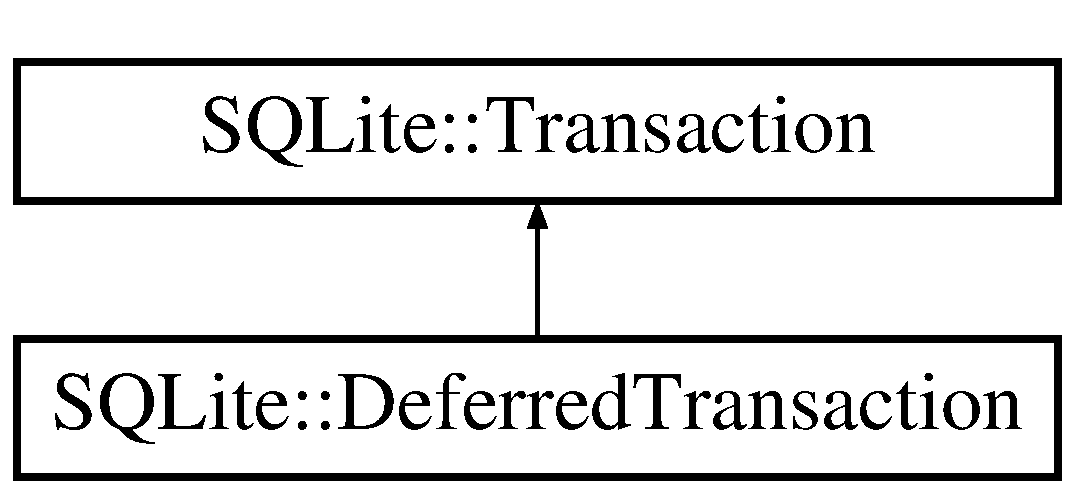
\includegraphics[height=2.000000cm]{class_s_q_lite_1_1_deferred_transaction}
\end{center}
\end{figure}
\subsection*{Public Member Functions}
\begin{DoxyCompactItemize}
\item 
\hypertarget{class_s_q_lite_1_1_deferred_transaction_ae1b880ce4c3796565b6ea4d492f61202}{{\bfseries Deferred\-Transaction} (\hyperlink{class_s_q_lite_1_1_d_b_connection}{D\-B\-Connection} \&connection)}\label{class_s_q_lite_1_1_deferred_transaction_ae1b880ce4c3796565b6ea4d492f61202}

\end{DoxyCompactItemize}
\subsection*{Additional Inherited Members}


The documentation for this class was generated from the following file\-:\begin{DoxyCompactItemize}
\item 
src/Transaction.\-h\end{DoxyCompactItemize}

\hypertarget{class_s_q_lite_1_1_exception}{\section{S\-Q\-Lite\-:\-:Exception Class Reference}
\label{class_s_q_lite_1_1_exception}\index{S\-Q\-Lite\-::\-Exception@{S\-Q\-Lite\-::\-Exception}}
}


Encapsulation of the error code and message from S\-Q\-Lite3, based on std\-::runtime\-\_\-error.  




{\ttfamily \#include $<$Exception.\-h$>$}

Inheritance diagram for S\-Q\-Lite\-:\-:Exception\-:\begin{figure}[H]
\begin{center}
\leavevmode
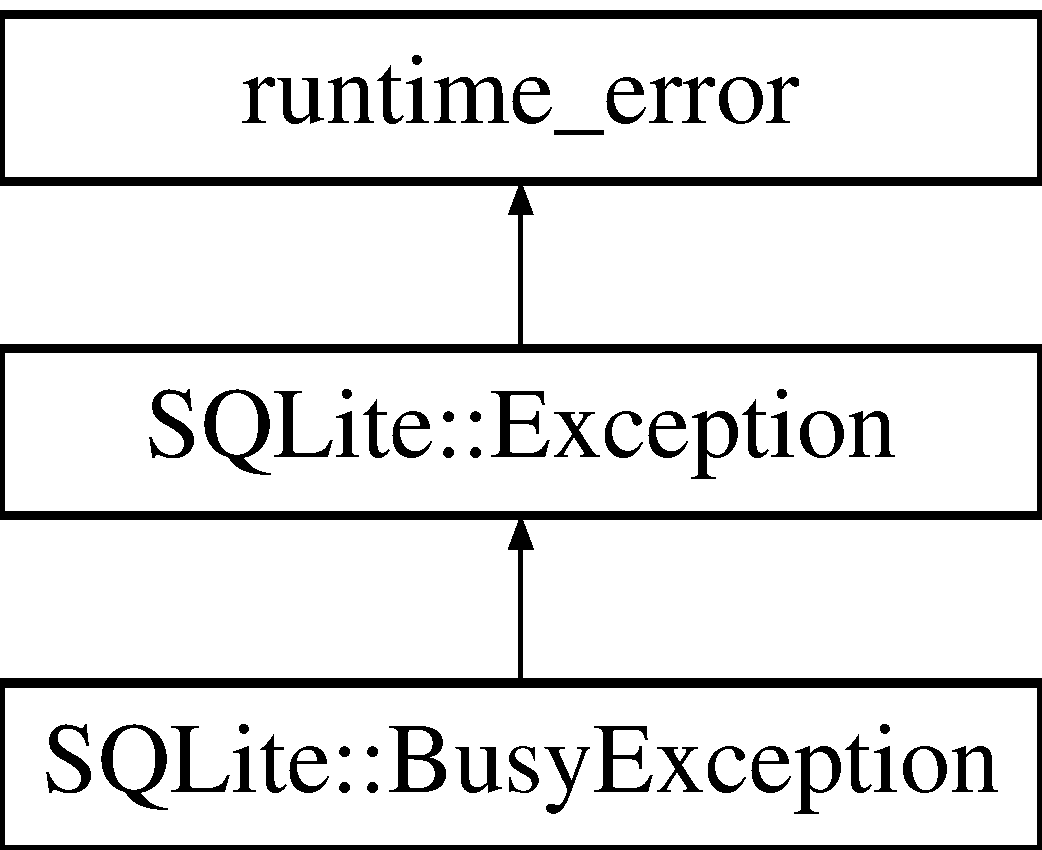
\includegraphics[height=3.000000cm]{class_s_q_lite_1_1_exception}
\end{center}
\end{figure}
\subsection*{Public Member Functions}
\begin{DoxyCompactItemize}
\item 
\hypertarget{class_s_q_lite_1_1_exception_a55056f0e661e2d0c09160404a7260d13}{{\bfseries Exception} (sqlite3 $\ast$const connection)}\label{class_s_q_lite_1_1_exception_a55056f0e661e2d0c09160404a7260d13}

\item 
\hypertarget{class_s_q_lite_1_1_exception_a7b00f63c9d211ea199ad06f184185a07}{{\bfseries Exception} (const int code, const std\-::string \&message)}\label{class_s_q_lite_1_1_exception_a7b00f63c9d211ea199ad06f184185a07}

\end{DoxyCompactItemize}
\subsection*{Public Attributes}
\begin{DoxyCompactItemize}
\item 
\hypertarget{class_s_q_lite_1_1_exception_aba01c386c828c7bd856c1691168aae2e}{const int {\bfseries errcode}}\label{class_s_q_lite_1_1_exception_aba01c386c828c7bd856c1691168aae2e}

\item 
\hypertarget{class_s_q_lite_1_1_exception_a4143712e07629a2d5097039e55189486}{const std\-::string {\bfseries message}}\label{class_s_q_lite_1_1_exception_a4143712e07629a2d5097039e55189486}

\end{DoxyCompactItemize}


\subsection{Detailed Description}
Encapsulation of the error code and message from S\-Q\-Lite3, based on std\-::runtime\-\_\-error. 



The documentation for this class was generated from the following file\-:\begin{DoxyCompactItemize}
\item 
src/Exception.\-h\end{DoxyCompactItemize}

\hypertarget{class_s_q_lite_1_1_exclusive_transaction}{\section{S\-Q\-Lite\-:\-:Exclusive\-Transaction Class Reference}
\label{class_s_q_lite_1_1_exclusive_transaction}\index{S\-Q\-Lite\-::\-Exclusive\-Transaction@{S\-Q\-Lite\-::\-Exclusive\-Transaction}}
}
Inheritance diagram for S\-Q\-Lite\-:\-:Exclusive\-Transaction\-:\begin{figure}[H]
\begin{center}
\leavevmode
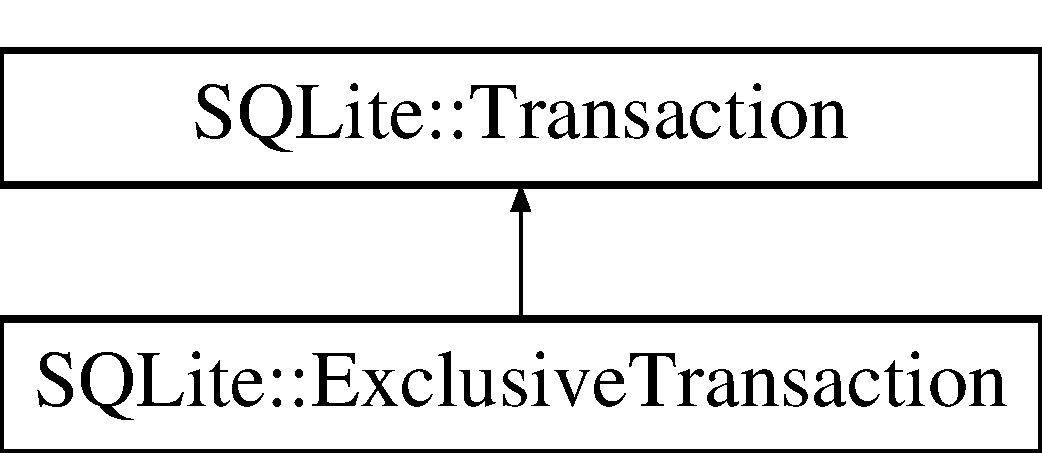
\includegraphics[height=2.000000cm]{class_s_q_lite_1_1_exclusive_transaction}
\end{center}
\end{figure}
\subsection*{Public Member Functions}
\begin{DoxyCompactItemize}
\item 
\hypertarget{class_s_q_lite_1_1_exclusive_transaction_a70f16f1e9764fd35b0c7e9fbf7314a1f}{{\bfseries Exclusive\-Transaction} (\hyperlink{class_s_q_lite_1_1_d_b_connection}{D\-B\-Connection} \&connection)}\label{class_s_q_lite_1_1_exclusive_transaction_a70f16f1e9764fd35b0c7e9fbf7314a1f}

\end{DoxyCompactItemize}
\subsection*{Additional Inherited Members}


The documentation for this class was generated from the following file\-:\begin{DoxyCompactItemize}
\item 
src/Transaction.\-h\end{DoxyCompactItemize}

\hypertarget{struct_s_q_lite_1_1function__traits}{\section{S\-Q\-Lite\-:\-:function\-\_\-traits$<$ T $>$ Struct Template Reference}
\label{struct_s_q_lite_1_1function__traits}\index{S\-Q\-Lite\-::function\-\_\-traits$<$ T $>$@{S\-Q\-Lite\-::function\-\_\-traits$<$ T $>$}}
}


The documentation for this struct was generated from the following file\-:\begin{DoxyCompactItemize}
\item 
src/Functions.\-h\end{DoxyCompactItemize}

\hypertarget{struct_s_q_lite_1_1function__traits_3_01_r_07_6_08_07_args_8_8_8_08_4}{\section{S\-Q\-Lite\-:\-:function\-\_\-traits$<$ R(\&)(Args...)$>$ Struct Template Reference}
\label{struct_s_q_lite_1_1function__traits_3_01_r_07_6_08_07_args_8_8_8_08_4}\index{S\-Q\-Lite\-::function\-\_\-traits$<$ R(\&)(\-Args...)$>$@{S\-Q\-Lite\-::function\-\_\-traits$<$ R(\&)(\-Args...)$>$}}
}
\subsection*{Classes}
\begin{DoxyCompactItemize}
\item 
struct \hyperlink{struct_s_q_lite_1_1function__traits_3_01_r_07_6_08_07_args_8_8_8_08_4_1_1arg}{arg}
\end{DoxyCompactItemize}
\subsection*{Public Types}
\begin{DoxyCompactItemize}
\item 
\hypertarget{struct_s_q_lite_1_1function__traits_3_01_r_07_6_08_07_args_8_8_8_08_4_a3bf67e9e1ba669be8b00cec2d3b1b561}{typedef std\-::function$<$ R(Args...)$>$ {\bfseries f\-\_\-type}}\label{struct_s_q_lite_1_1function__traits_3_01_r_07_6_08_07_args_8_8_8_08_4_a3bf67e9e1ba669be8b00cec2d3b1b561}

\item 
\hypertarget{struct_s_q_lite_1_1function__traits_3_01_r_07_6_08_07_args_8_8_8_08_4_a6c7248a8112d42fb423a58b06fbae55d}{typedef R {\bfseries result\-\_\-type}}\label{struct_s_q_lite_1_1function__traits_3_01_r_07_6_08_07_args_8_8_8_08_4_a6c7248a8112d42fb423a58b06fbae55d}

\end{DoxyCompactItemize}
\subsection*{Static Public Attributes}
\begin{DoxyCompactItemize}
\item 
\hypertarget{struct_s_q_lite_1_1function__traits_3_01_r_07_6_08_07_args_8_8_8_08_4_a59d3074c935e3aadc124b83ed65a7cad}{static const size\-\_\-t {\bfseries nargs} = sizeof...(Args)}\label{struct_s_q_lite_1_1function__traits_3_01_r_07_6_08_07_args_8_8_8_08_4_a59d3074c935e3aadc124b83ed65a7cad}

\end{DoxyCompactItemize}


The documentation for this struct was generated from the following file\-:\begin{DoxyCompactItemize}
\item 
src/Functions.\-h\end{DoxyCompactItemize}

\hypertarget{struct_s_q_lite_1_1function__traits_3_01_r_07_5_08_07_args_8_8_8_08_4}{\section{S\-Q\-Lite\-:\-:function\-\_\-traits$<$ R($\ast$)(Args...)$>$ Struct Template Reference}
\label{struct_s_q_lite_1_1function__traits_3_01_r_07_5_08_07_args_8_8_8_08_4}\index{S\-Q\-Lite\-::function\-\_\-traits$<$ R($\ast$)(\-Args...)$>$@{S\-Q\-Lite\-::function\-\_\-traits$<$ R($\ast$)(\-Args...)$>$}}
}
\subsection*{Classes}
\begin{DoxyCompactItemize}
\item 
struct \hyperlink{struct_s_q_lite_1_1function__traits_3_01_r_07_5_08_07_args_8_8_8_08_4_1_1arg}{arg}
\end{DoxyCompactItemize}
\subsection*{Public Types}
\begin{DoxyCompactItemize}
\item 
\hypertarget{struct_s_q_lite_1_1function__traits_3_01_r_07_5_08_07_args_8_8_8_08_4_afcf9cc79ab2beea01be6a226df1e928d}{typedef std\-::function$<$ R(Args...)$>$ {\bfseries f\-\_\-type}}\label{struct_s_q_lite_1_1function__traits_3_01_r_07_5_08_07_args_8_8_8_08_4_afcf9cc79ab2beea01be6a226df1e928d}

\item 
\hypertarget{struct_s_q_lite_1_1function__traits_3_01_r_07_5_08_07_args_8_8_8_08_4_a85e42a040d0c12404d671e71d48a260d}{typedef R {\bfseries result\-\_\-type}}\label{struct_s_q_lite_1_1function__traits_3_01_r_07_5_08_07_args_8_8_8_08_4_a85e42a040d0c12404d671e71d48a260d}

\end{DoxyCompactItemize}
\subsection*{Static Public Attributes}
\begin{DoxyCompactItemize}
\item 
\hypertarget{struct_s_q_lite_1_1function__traits_3_01_r_07_5_08_07_args_8_8_8_08_4_afa9f09de2f05f1bb4280ce85a1aba027}{static const size\-\_\-t {\bfseries nargs} = sizeof...(Args)}\label{struct_s_q_lite_1_1function__traits_3_01_r_07_5_08_07_args_8_8_8_08_4_afa9f09de2f05f1bb4280ce85a1aba027}

\end{DoxyCompactItemize}


The documentation for this struct was generated from the following file\-:\begin{DoxyCompactItemize}
\item 
src/Functions.\-h\end{DoxyCompactItemize}

\hypertarget{struct_s_q_lite_1_1function__traits_3_01_r_07_c_1_1_5_08_07_args_8_8_8_08_01const_01_01_4}{\section{S\-Q\-Lite\-:\-:function\-\_\-traits$<$ R(C\-:\-:$\ast$)(Args...) const $>$ Struct Template Reference}
\label{struct_s_q_lite_1_1function__traits_3_01_r_07_c_1_1_5_08_07_args_8_8_8_08_01const_01_01_4}\index{S\-Q\-Lite\-::function\-\_\-traits$<$ R(\-C\-::$\ast$)(\-Args...) const  $>$@{S\-Q\-Lite\-::function\-\_\-traits$<$ R(\-C\-::$\ast$)(\-Args...) const  $>$}}
}
\subsection*{Classes}
\begin{DoxyCompactItemize}
\item 
struct \hyperlink{struct_s_q_lite_1_1function__traits_3_01_r_07_c_1_1_5_08_07_args_8_8_8_08_01const_01_01_4_1_1arg}{arg}
\end{DoxyCompactItemize}
\subsection*{Public Types}
\begin{DoxyCompactItemize}
\item 
\hypertarget{struct_s_q_lite_1_1function__traits_3_01_r_07_c_1_1_5_08_07_args_8_8_8_08_01const_01_01_4_a94a8a7aead0412d73a03e2f6f97f628d}{typedef std\-::function$<$ R(Args...)$>$ {\bfseries f\-\_\-type}}\label{struct_s_q_lite_1_1function__traits_3_01_r_07_c_1_1_5_08_07_args_8_8_8_08_01const_01_01_4_a94a8a7aead0412d73a03e2f6f97f628d}

\item 
\hypertarget{struct_s_q_lite_1_1function__traits_3_01_r_07_c_1_1_5_08_07_args_8_8_8_08_01const_01_01_4_abd8ad43b029985269496f0fb2166d690}{typedef R {\bfseries result\-\_\-type}}\label{struct_s_q_lite_1_1function__traits_3_01_r_07_c_1_1_5_08_07_args_8_8_8_08_01const_01_01_4_abd8ad43b029985269496f0fb2166d690}

\end{DoxyCompactItemize}
\subsection*{Static Public Attributes}
\begin{DoxyCompactItemize}
\item 
\hypertarget{struct_s_q_lite_1_1function__traits_3_01_r_07_c_1_1_5_08_07_args_8_8_8_08_01const_01_01_4_a72dae0c2818d49446c007795e9aadc35}{static const size\-\_\-t {\bfseries nargs} = sizeof...(Args)}\label{struct_s_q_lite_1_1function__traits_3_01_r_07_c_1_1_5_08_07_args_8_8_8_08_01const_01_01_4_a72dae0c2818d49446c007795e9aadc35}

\end{DoxyCompactItemize}


The documentation for this struct was generated from the following file\-:\begin{DoxyCompactItemize}
\item 
src/Functions.\-h\end{DoxyCompactItemize}

\hypertarget{struct_s_q_lite_1_1function__traits_3_01_r_07_c_1_1_5_08_07_args_8_8_8_08_4}{\section{S\-Q\-Lite\-:\-:function\-\_\-traits$<$ R(C\-:\-:$\ast$)(Args...)$>$ Struct Template Reference}
\label{struct_s_q_lite_1_1function__traits_3_01_r_07_c_1_1_5_08_07_args_8_8_8_08_4}\index{S\-Q\-Lite\-::function\-\_\-traits$<$ R(\-C\-::$\ast$)(\-Args...)$>$@{S\-Q\-Lite\-::function\-\_\-traits$<$ R(\-C\-::$\ast$)(\-Args...)$>$}}
}
\subsection*{Classes}
\begin{DoxyCompactItemize}
\item 
struct \hyperlink{struct_s_q_lite_1_1function__traits_3_01_r_07_c_1_1_5_08_07_args_8_8_8_08_4_1_1arg}{arg}
\end{DoxyCompactItemize}
\subsection*{Public Types}
\begin{DoxyCompactItemize}
\item 
\hypertarget{struct_s_q_lite_1_1function__traits_3_01_r_07_c_1_1_5_08_07_args_8_8_8_08_4_a672d67d6e5525c90ed5b4c28e4f2514c}{typedef std\-::function$<$ R(Args...)$>$ {\bfseries f\-\_\-type}}\label{struct_s_q_lite_1_1function__traits_3_01_r_07_c_1_1_5_08_07_args_8_8_8_08_4_a672d67d6e5525c90ed5b4c28e4f2514c}

\item 
\hypertarget{struct_s_q_lite_1_1function__traits_3_01_r_07_c_1_1_5_08_07_args_8_8_8_08_4_ae15055764604ef8c9693d73f28f018e6}{typedef R {\bfseries result\-\_\-type}}\label{struct_s_q_lite_1_1function__traits_3_01_r_07_c_1_1_5_08_07_args_8_8_8_08_4_ae15055764604ef8c9693d73f28f018e6}

\end{DoxyCompactItemize}
\subsection*{Static Public Attributes}
\begin{DoxyCompactItemize}
\item 
\hypertarget{struct_s_q_lite_1_1function__traits_3_01_r_07_c_1_1_5_08_07_args_8_8_8_08_4_aa14cf5fc72021d00d74eec8b1da2c6c2}{static const size\-\_\-t {\bfseries nargs} = sizeof...(Args)}\label{struct_s_q_lite_1_1function__traits_3_01_r_07_c_1_1_5_08_07_args_8_8_8_08_4_aa14cf5fc72021d00d74eec8b1da2c6c2}

\end{DoxyCompactItemize}


The documentation for this struct was generated from the following file\-:\begin{DoxyCompactItemize}
\item 
src/Functions.\-h\end{DoxyCompactItemize}

\hypertarget{class_s_q_lite_1_1_immediate_transaction}{\section{S\-Q\-Lite\-:\-:Immediate\-Transaction Class Reference}
\label{class_s_q_lite_1_1_immediate_transaction}\index{S\-Q\-Lite\-::\-Immediate\-Transaction@{S\-Q\-Lite\-::\-Immediate\-Transaction}}
}
Inheritance diagram for S\-Q\-Lite\-:\-:Immediate\-Transaction\-:\begin{figure}[H]
\begin{center}
\leavevmode
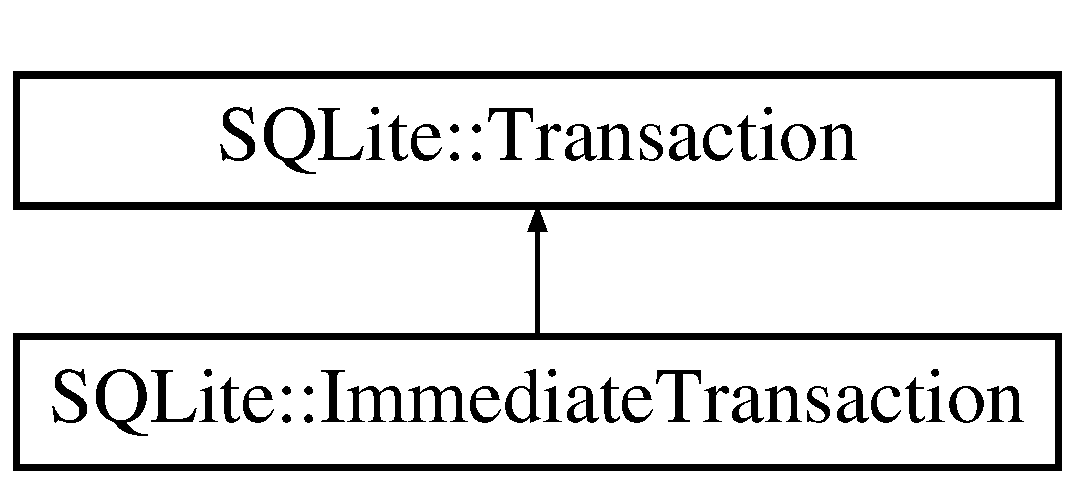
\includegraphics[height=2.000000cm]{class_s_q_lite_1_1_immediate_transaction}
\end{center}
\end{figure}
\subsection*{Public Member Functions}
\begin{DoxyCompactItemize}
\item 
\hypertarget{class_s_q_lite_1_1_immediate_transaction_a3c6f88a4f4f6b299461c4a30a79b17e1}{{\bfseries Immediate\-Transaction} (\hyperlink{class_s_q_lite_1_1_d_b_connection}{D\-B\-Connection} \&connection)}\label{class_s_q_lite_1_1_immediate_transaction_a3c6f88a4f4f6b299461c4a30a79b17e1}

\end{DoxyCompactItemize}
\subsection*{Additional Inherited Members}


The documentation for this class was generated from the following file\-:\begin{DoxyCompactItemize}
\item 
src/Transaction.\-h\end{DoxyCompactItemize}

\hypertarget{structstd_1_1is__placeholder_3_01_s_q_lite_1_1placeholder__template_3_01_n_01_4_01_4}{\section{std\-:\-:is\-\_\-placeholder$<$ S\-Q\-Lite\-:\-:placeholder\-\_\-template$<$ N $>$ $>$ Struct Template Reference}
\label{structstd_1_1is__placeholder_3_01_s_q_lite_1_1placeholder__template_3_01_n_01_4_01_4}\index{std\-::is\-\_\-placeholder$<$ S\-Q\-Lite\-::placeholder\-\_\-template$<$ N $>$ $>$@{std\-::is\-\_\-placeholder$<$ S\-Q\-Lite\-::placeholder\-\_\-template$<$ N $>$ $>$}}
}
Inheritance diagram for std\-:\-:is\-\_\-placeholder$<$ S\-Q\-Lite\-:\-:placeholder\-\_\-template$<$ N $>$ $>$\-:\begin{figure}[H]
\begin{center}
\leavevmode
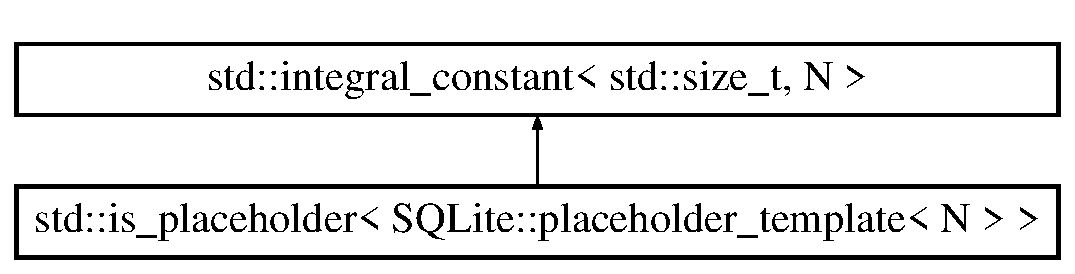
\includegraphics[height=2.000000cm]{structstd_1_1is__placeholder_3_01_s_q_lite_1_1placeholder__template_3_01_n_01_4_01_4}
\end{center}
\end{figure}


The documentation for this struct was generated from the following file\-:\begin{DoxyCompactItemize}
\item 
src/Functions.\-h\end{DoxyCompactItemize}

\hypertarget{class_s_q_lite_1_1_lock}{\section{S\-Q\-Lite\-:\-:Lock Class Reference}
\label{class_s_q_lite_1_1_lock}\index{S\-Q\-Lite\-::\-Lock@{S\-Q\-Lite\-::\-Lock}}
}


Locks the given \hyperlink{class_s_q_lite_1_1_mutex}{Mutex}.  




{\ttfamily \#include $<$Mutex.\-h$>$}

\subsection*{Public Member Functions}
\begin{DoxyCompactItemize}
\item 
\hypertarget{class_s_q_lite_1_1_lock_ad7c333c305ff20ce19959ef2b0d8a6b7}{{\bfseries Lock} (const \hyperlink{class_s_q_lite_1_1_mutex}{Mutex} \&m)}\label{class_s_q_lite_1_1_lock_ad7c333c305ff20ce19959ef2b0d8a6b7}

\end{DoxyCompactItemize}


\subsection{Detailed Description}
Locks the given \hyperlink{class_s_q_lite_1_1_mutex}{Mutex}. 

Uses R\-A\-I\-I to help with locking and unlocking the given \hyperlink{class_s_q_lite_1_1_mutex}{Mutex}. 

The documentation for this class was generated from the following files\-:\begin{DoxyCompactItemize}
\item 
src/Mutex.\-h\item 
src/Mutex.\-cpp\end{DoxyCompactItemize}

\hypertarget{class_s_q_lite_1_1_mutex}{\section{S\-Q\-Lite\-:\-:Mutex Class Reference}
\label{class_s_q_lite_1_1_mutex}\index{S\-Q\-Lite\-::\-Mutex@{S\-Q\-Lite\-::\-Mutex}}
}


Helps with serializing access to a database connection.  




{\ttfamily \#include $<$Mutex.\-h$>$}

\subsection*{Public Member Functions}
\begin{DoxyCompactItemize}
\item 
\hypertarget{class_s_q_lite_1_1_mutex_ad98ed6e326082828a5860cc037683bd1}{{\bfseries Mutex} (sqlite3\-\_\-mutex $\ast$mutex)}\label{class_s_q_lite_1_1_mutex_ad98ed6e326082828a5860cc037683bd1}

\item 
\hypertarget{class_s_q_lite_1_1_mutex_a56ba1f0c1411940ab52279497d15812a}{void \hyperlink{class_s_q_lite_1_1_mutex_a56ba1f0c1411940ab52279497d15812a}{lock} () noexcept}\label{class_s_q_lite_1_1_mutex_a56ba1f0c1411940ab52279497d15812a}

\begin{DoxyCompactList}\small\item\em Locks the mutex, blocks if the mutex is not available. \end{DoxyCompactList}\item 
bool \hyperlink{class_s_q_lite_1_1_mutex_a95b5ebd5fef0bd37b30e3867d60389f8}{try\-Lock} () noexcept
\begin{DoxyCompactList}\small\item\em Tries to lock the mutex, returns if the mutex is not available. \end{DoxyCompactList}\item 
\hypertarget{class_s_q_lite_1_1_mutex_ad9238aeb94205ac18d67c9652dcc6ef9}{void \hyperlink{class_s_q_lite_1_1_mutex_ad9238aeb94205ac18d67c9652dcc6ef9}{unlock} () noexcept}\label{class_s_q_lite_1_1_mutex_ad9238aeb94205ac18d67c9652dcc6ef9}

\begin{DoxyCompactList}\small\item\em Unlocks the mutex. \end{DoxyCompactList}\end{DoxyCompactItemize}


\subsection{Detailed Description}
Helps with serializing access to a database connection. 

Mutexes are only useful when threading mode is set to \char`\"{}\-Serialized\char`\"{}. 

\subsection{Member Function Documentation}
\hypertarget{class_s_q_lite_1_1_mutex_a95b5ebd5fef0bd37b30e3867d60389f8}{\index{S\-Q\-Lite\-::\-Mutex@{S\-Q\-Lite\-::\-Mutex}!try\-Lock@{try\-Lock}}
\index{try\-Lock@{try\-Lock}!SQLite::Mutex@{S\-Q\-Lite\-::\-Mutex}}
\subsubsection[{try\-Lock}]{\setlength{\rightskip}{0pt plus 5cm}bool S\-Q\-Lite\-::\-Mutex\-::try\-Lock (
\begin{DoxyParamCaption}
{}
\end{DoxyParamCaption}
)\hspace{0.3cm}{\ttfamily [noexcept]}}}\label{class_s_q_lite_1_1_mutex_a95b5ebd5fef0bd37b30e3867d60389f8}


Tries to lock the mutex, returns if the mutex is not available. 

\begin{DoxyReturn}{Returns}
True if able to obtain lock. False otherwise. 
\end{DoxyReturn}


The documentation for this class was generated from the following files\-:\begin{DoxyCompactItemize}
\item 
src/Mutex.\-h\item 
src/Mutex.\-cpp\end{DoxyCompactItemize}

\hypertarget{struct_s_q_lite_1_1placeholder__template}{\section{S\-Q\-Lite\-:\-:placeholder\-\_\-template$<$ N $>$ Struct Template Reference}
\label{struct_s_q_lite_1_1placeholder__template}\index{S\-Q\-Lite\-::placeholder\-\_\-template$<$ N $>$@{S\-Q\-Lite\-::placeholder\-\_\-template$<$ N $>$}}
}
\subsection*{Static Public Attributes}
\begin{DoxyCompactItemize}
\item 
\hypertarget{struct_s_q_lite_1_1placeholder__template_a60819a986742f08edbfc535124c006b1}{static \hyperlink{struct_s_q_lite_1_1placeholder__template}{placeholder\-\_\-template} {\bfseries pt}}\label{struct_s_q_lite_1_1placeholder__template_a60819a986742f08edbfc535124c006b1}

\end{DoxyCompactItemize}


The documentation for this struct was generated from the following file\-:\begin{DoxyCompactItemize}
\item 
src/Functions.\-h\end{DoxyCompactItemize}

\hypertarget{class_s_q_lite_1_1_reader}{\section{S\-Q\-Lite\-:\-:Reader$<$ T $>$ Class Template Reference}
\label{class_s_q_lite_1_1_reader}\index{S\-Q\-Lite\-::\-Reader$<$ T $>$@{S\-Q\-Lite\-::\-Reader$<$ T $>$}}
}
\subsection*{Public Member Functions}
\begin{DoxyCompactItemize}
\item 
\hypertarget{class_s_q_lite_1_1_reader_a82c5bc45048b8328a2fcc9bb4ff975f2}{int {\bfseries get\-Int} (const int column) const noexcept}\label{class_s_q_lite_1_1_reader_a82c5bc45048b8328a2fcc9bb4ff975f2}

\item 
\hypertarget{class_s_q_lite_1_1_reader_a87dd8234c2bd5f19466813f8a68ab80a}{int {\bfseries get\-Int} (const std\-::string \&name) const noexcept}\label{class_s_q_lite_1_1_reader_a87dd8234c2bd5f19466813f8a68ab80a}

\item 
\hypertarget{class_s_q_lite_1_1_reader_adb7b9705a4638d6d5af5ca26dfa474ff}{int64\-\_\-t {\bfseries get\-Int64} (const int column) const noexcept}\label{class_s_q_lite_1_1_reader_adb7b9705a4638d6d5af5ca26dfa474ff}

\item 
\hypertarget{class_s_q_lite_1_1_reader_aea6d24bb9247bfc52fe77d62be961dd2}{int64\-\_\-t {\bfseries get\-Int64} (const std\-::string \&name) const noexcept}\label{class_s_q_lite_1_1_reader_aea6d24bb9247bfc52fe77d62be961dd2}

\item 
\hypertarget{class_s_q_lite_1_1_reader_a971fb706b9215a89532ac48640f94832}{unsigned int {\bfseries get\-U\-Int} (const int column) const noexcept}\label{class_s_q_lite_1_1_reader_a971fb706b9215a89532ac48640f94832}

\item 
\hypertarget{class_s_q_lite_1_1_reader_a18315a8379249158c3f827441e8f6de0}{unsigned int {\bfseries get\-U\-Int} (const std\-::string \&name) const noexcept}\label{class_s_q_lite_1_1_reader_a18315a8379249158c3f827441e8f6de0}

\item 
\hypertarget{class_s_q_lite_1_1_reader_a679e56078c78e01c99fa08ad0b7ee782}{double {\bfseries get\-Double} (const int column) const noexcept}\label{class_s_q_lite_1_1_reader_a679e56078c78e01c99fa08ad0b7ee782}

\item 
\hypertarget{class_s_q_lite_1_1_reader_a45e9dd813439e8cda7608e18c1ccce5f}{double {\bfseries get\-Double} (const std\-::string \&name) const noexcept}\label{class_s_q_lite_1_1_reader_a45e9dd813439e8cda7608e18c1ccce5f}

\item 
\hypertarget{class_s_q_lite_1_1_reader_a80028dc9f221648fe2398b40bd380c31}{const \hyperlink{class_s_q_lite_1_1_blob}{Blob} {\bfseries get\-Blob} (const int column) const noexcept}\label{class_s_q_lite_1_1_reader_a80028dc9f221648fe2398b40bd380c31}

\item 
\hypertarget{class_s_q_lite_1_1_reader_a4e50d9ec365c547b5edb7d062aeba72b}{const \hyperlink{class_s_q_lite_1_1_blob}{Blob} {\bfseries get\-Blob} (const std\-::string \&name) const noexcept}\label{class_s_q_lite_1_1_reader_a4e50d9ec365c547b5edb7d062aeba72b}

\item 
\hypertarget{class_s_q_lite_1_1_reader_a0920d021f6962f75e7b555e3f20fc0fc}{const std\-::string {\bfseries get\-String} (const int column) const noexcept}\label{class_s_q_lite_1_1_reader_a0920d021f6962f75e7b555e3f20fc0fc}

\item 
\hypertarget{class_s_q_lite_1_1_reader_a44f9f5da46aa91b869fe26a188e803fa}{const std\-::string {\bfseries get\-String} (const std\-::string \&name) const noexcept}\label{class_s_q_lite_1_1_reader_a44f9f5da46aa91b869fe26a188e803fa}

\item 
\hypertarget{class_s_q_lite_1_1_reader_a2b48f9e2ffbcfe787d85b4372a7ee29d}{const std\-::u16string {\bfseries get\-U16\-String} (const int column) const noexcept}\label{class_s_q_lite_1_1_reader_a2b48f9e2ffbcfe787d85b4372a7ee29d}

\item 
\hypertarget{class_s_q_lite_1_1_reader_ad6024ad6e74ee1ac47ad0ce79f905026}{const std\-::u16string {\bfseries get\-U16\-String} (const std\-::string \&name) const noexcept}\label{class_s_q_lite_1_1_reader_ad6024ad6e74ee1ac47ad0ce79f905026}

\item 
\hypertarget{class_s_q_lite_1_1_reader_aeb571e9157ef46c42ed48fc229b7842d}{int {\bfseries get\-Bytes} (const int column) const noexcept}\label{class_s_q_lite_1_1_reader_aeb571e9157ef46c42ed48fc229b7842d}

\item 
\hypertarget{class_s_q_lite_1_1_reader_ad183a562774f9590273bf35c6e232a1a}{int {\bfseries get\-Bytes} (const std\-::string \&name) const noexcept}\label{class_s_q_lite_1_1_reader_ad183a562774f9590273bf35c6e232a1a}

\item 
\hypertarget{class_s_q_lite_1_1_reader_a0450ea397b1a9d8dd636b82c8757d33e}{Type {\bfseries get\-Type} (const int column) const noexcept}\label{class_s_q_lite_1_1_reader_a0450ea397b1a9d8dd636b82c8757d33e}

\item 
\hypertarget{class_s_q_lite_1_1_reader_ae4f049a45c69b9e1bf6db4cf63699f64}{Type {\bfseries get\-Type} (const std\-::string \&name) const noexcept}\label{class_s_q_lite_1_1_reader_ae4f049a45c69b9e1bf6db4cf63699f64}

\item 
\hypertarget{class_s_q_lite_1_1_reader_a41fcbc5da6eb3fe6fc75e4faed208fc6}{\hyperlink{class_s_q_lite_1_1_value}{Value} {\bfseries get\-Value} (const int column) const noexcept}\label{class_s_q_lite_1_1_reader_a41fcbc5da6eb3fe6fc75e4faed208fc6}

\item 
\hypertarget{class_s_q_lite_1_1_reader_ad352a7124ee46d756462c8a1b014599a}{\hyperlink{class_s_q_lite_1_1_value}{Value} {\bfseries get\-Value} (const std\-::string \&name) const }\label{class_s_q_lite_1_1_reader_ad352a7124ee46d756462c8a1b014599a}

\item 
\hypertarget{class_s_q_lite_1_1_reader_a9e6b9d0d99dea8964a34a3c2f08e99bc}{int {\bfseries get\-Column\-Count} () const noexcept}\label{class_s_q_lite_1_1_reader_a9e6b9d0d99dea8964a34a3c2f08e99bc}

\item 
\hypertarget{class_s_q_lite_1_1_reader_a5004961d65336631d45de411ffb87cd5}{const char $\ast$ {\bfseries get\-Column\-Name} (const int index) const noexcept}\label{class_s_q_lite_1_1_reader_a5004961d65336631d45de411ffb87cd5}

\item 
\hypertarget{class_s_q_lite_1_1_reader_a3b220314921864971914abe137e58013}{const char $\ast$ {\bfseries get\-Column\-Wide\-Name} (const int index) const noexcept}\label{class_s_q_lite_1_1_reader_a3b220314921864971914abe137e58013}

\item 
int \hyperlink{class_s_q_lite_1_1_reader_ae7eaa050a97cda893e9737bca416f0cb}{get\-Column\-Index} (const std\-::string \&name) const 
\end{DoxyCompactItemize}


\subsection{Member Function Documentation}
\hypertarget{class_s_q_lite_1_1_reader_ae7eaa050a97cda893e9737bca416f0cb}{\index{S\-Q\-Lite\-::\-Reader@{S\-Q\-Lite\-::\-Reader}!get\-Column\-Index@{get\-Column\-Index}}
\index{get\-Column\-Index@{get\-Column\-Index}!SQLite::Reader@{S\-Q\-Lite\-::\-Reader}}
\subsubsection[{get\-Column\-Index}]{\setlength{\rightskip}{0pt plus 5cm}template$<$typename T$>$ int {\bf S\-Q\-Lite\-::\-Reader}$<$ T $>$\-::get\-Column\-Index (
\begin{DoxyParamCaption}
\item[{const std\-::string \&}]{name}
\end{DoxyParamCaption}
) const\hspace{0.3cm}{\ttfamily [inline]}}}\label{class_s_q_lite_1_1_reader_ae7eaa050a97cda893e9737bca416f0cb}

\begin{DoxyExceptions}{Exceptions}
{\em \hyperlink{class_s_q_lite_1_1_s_q_lite_x_x_exception}{S\-Q\-Lite\-X\-X\-Exception}} & if no column with specified name was found \\
\hline
\end{DoxyExceptions}


The documentation for this class was generated from the following file\-:\begin{DoxyCompactItemize}
\item 
src/Statement.\-h\end{DoxyCompactItemize}

\hypertarget{class_s_q_lite_1_1_row}{\section{S\-Q\-Lite\-:\-:Row Class Reference}
\label{class_s_q_lite_1_1_row}\index{S\-Q\-Lite\-::\-Row@{S\-Q\-Lite\-::\-Row}}
}


Represents a returned row when stepping through a \char`\"{}\-S\-E\-L\-E\-C\-T\char`\"{} statement.  




{\ttfamily \#include $<$Statement.\-h$>$}

Inheritance diagram for S\-Q\-Lite\-:\-:Row\-:\begin{figure}[H]
\begin{center}
\leavevmode
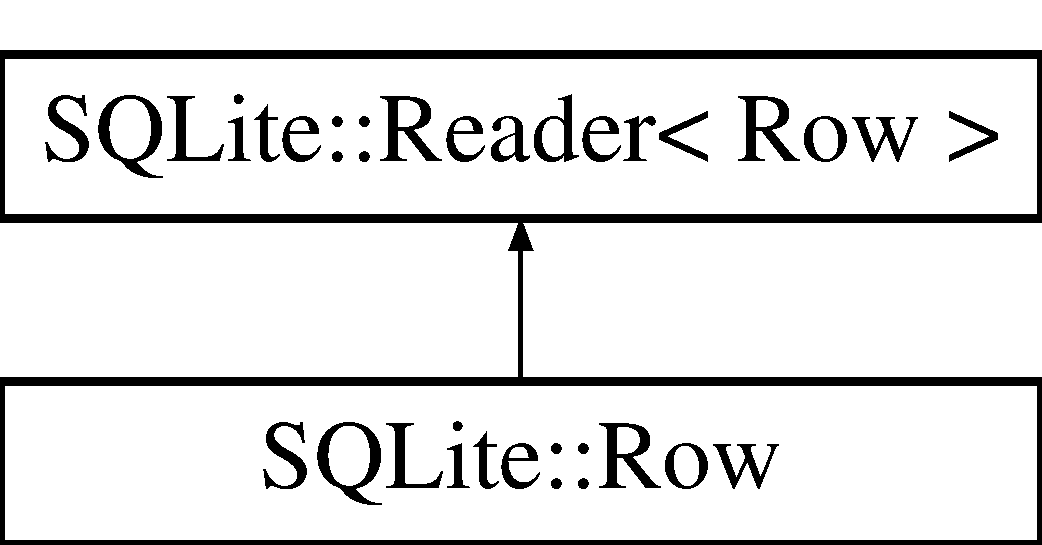
\includegraphics[height=2.000000cm]{class_s_q_lite_1_1_row}
\end{center}
\end{figure}
\subsection*{Public Member Functions}
\begin{DoxyCompactItemize}
\item 
\hypertarget{class_s_q_lite_1_1_row_a0cdd34663266ff8c19ee1313a87d51f0}{sqlite3\-\_\-stmt $\ast$ \hyperlink{class_s_q_lite_1_1_row_a0cdd34663266ff8c19ee1313a87d51f0}{get\-Handle} () const noexcept}\label{class_s_q_lite_1_1_row_a0cdd34663266ff8c19ee1313a87d51f0}

\begin{DoxyCompactList}\small\item\em Returns pointer to the underlying \char`\"{}sqlite3\-\_\-stmt\char`\"{} object. \end{DoxyCompactList}\item 
\hypertarget{class_s_q_lite_1_1_row_ac93d6eec191f8f92ce72f481935d1832}{{\bfseries Row} (sqlite3\-\_\-stmt $\ast$const statement) noexcept}\label{class_s_q_lite_1_1_row_ac93d6eec191f8f92ce72f481935d1832}

\item 
\hypertarget{class_s_q_lite_1_1_row_a82ca0ee6352667cc9f6d41972dedd5a6}{\hyperlink{class_s_q_lite_1_1_value}{Value} {\bfseries operator\mbox{[}$\,$\mbox{]}} (int column) const }\label{class_s_q_lite_1_1_row_a82ca0ee6352667cc9f6d41972dedd5a6}

\end{DoxyCompactItemize}


\subsection{Detailed Description}
Represents a returned row when stepping through a \char`\"{}\-S\-E\-L\-E\-C\-T\char`\"{} statement. 



The documentation for this class was generated from the following file\-:\begin{DoxyCompactItemize}
\item 
src/Statement.\-h\end{DoxyCompactItemize}

\hypertarget{class_s_q_lite_1_1_row_iterator}{\section{S\-Q\-Lite\-:\-:Row\-Iterator Class Reference}
\label{class_s_q_lite_1_1_row_iterator}\index{S\-Q\-Lite\-::\-Row\-Iterator@{S\-Q\-Lite\-::\-Row\-Iterator}}
}


Helps when iterating over rows in a \char`\"{}\-S\-E\-L\-E\-C\-T\char`\"{} statement.  




{\ttfamily \#include $<$Statement.\-h$>$}

\subsection*{Public Member Functions}
\begin{DoxyCompactItemize}
\item 
\hypertarget{class_s_q_lite_1_1_row_iterator_ad3927378b109ab3dfd6f86d8326f609c}{{\bfseries Row\-Iterator} (const \hyperlink{class_s_q_lite_1_1_statement}{Statement} \&statement) noexcept}\label{class_s_q_lite_1_1_row_iterator_ad3927378b109ab3dfd6f86d8326f609c}

\item 
\hypertarget{class_s_q_lite_1_1_row_iterator_a55c22680d983bd87d068bb304dbb1508}{\hyperlink{class_s_q_lite_1_1_row_iterator}{Row\-Iterator} \& {\bfseries operator++} () noexcept}\label{class_s_q_lite_1_1_row_iterator_a55c22680d983bd87d068bb304dbb1508}

\item 
\hypertarget{class_s_q_lite_1_1_row_iterator_ab5a2045335ee19bb897381b51b013a48}{bool {\bfseries operator!=} (const \hyperlink{class_s_q_lite_1_1_row_iterator}{Row\-Iterator} \&other) const noexcept}\label{class_s_q_lite_1_1_row_iterator_ab5a2045335ee19bb897381b51b013a48}

\item 
\hypertarget{class_s_q_lite_1_1_row_iterator_a1e27980d666a42f9835c919f8b9c93b1}{\hyperlink{class_s_q_lite_1_1_row}{Row} {\bfseries operator$\ast$} () const noexcept}\label{class_s_q_lite_1_1_row_iterator_a1e27980d666a42f9835c919f8b9c93b1}

\end{DoxyCompactItemize}


\subsection{Detailed Description}
Helps when iterating over rows in a \char`\"{}\-S\-E\-L\-E\-C\-T\char`\"{} statement. 

The documentation for this class was generated from the following files\-:\begin{DoxyCompactItemize}
\item 
src/Statement.\-h\item 
src/Statement.\-cpp\end{DoxyCompactItemize}

\hypertarget{struct_s_q_lite_1_1_s_q_lite_function_traits}{\section{S\-Q\-Lite\-:\-:S\-Q\-Lite\-Function\-Traits$<$ T $>$ Struct Template Reference}
\label{struct_s_q_lite_1_1_s_q_lite_function_traits}\index{S\-Q\-Lite\-::\-S\-Q\-Lite\-Function\-Traits$<$ T $>$@{S\-Q\-Lite\-::\-S\-Q\-Lite\-Function\-Traits$<$ T $>$}}
}


The documentation for this struct was generated from the following file\-:\begin{DoxyCompactItemize}
\item 
src/Functions.\-h\end{DoxyCompactItemize}

\hypertarget{struct_s_q_lite_1_1_s_q_lite_function_traits_3_01_r_07_6_08_07const_01std_1_1vector_3_01_value_01_4_01_6_08_4}{\section{S\-Q\-Lite\-:\-:S\-Q\-Lite\-Function\-Traits$<$ R(\&)(const std\-:\-:vector$<$ Value $>$ \&)$>$ Struct Template Reference}
\label{struct_s_q_lite_1_1_s_q_lite_function_traits_3_01_r_07_6_08_07const_01std_1_1vector_3_01_value_01_4_01_6_08_4}\index{S\-Q\-Lite\-::\-S\-Q\-Lite\-Function\-Traits$<$ R(\&)(const std\-::vector$<$ Value $>$ \&)$>$@{S\-Q\-Lite\-::\-S\-Q\-Lite\-Function\-Traits$<$ R(\&)(const std\-::vector$<$ Value $>$ \&)$>$}}
}
\subsection*{Public Types}
\begin{DoxyCompactItemize}
\item 
\hypertarget{struct_s_q_lite_1_1_s_q_lite_function_traits_3_01_r_07_6_08_07const_01std_1_1vector_3_01_value_01_4_01_6_08_4_a8687ea41557a72ddaf61ce3f076a5317}{typedef std\-::function$<$ R(const \\*
std\-::vector$<$ \hyperlink{class_s_q_lite_1_1_value}{Value} $>$ \&)$>$ {\bfseries f\-\_\-type}}\label{struct_s_q_lite_1_1_s_q_lite_function_traits_3_01_r_07_6_08_07const_01std_1_1vector_3_01_value_01_4_01_6_08_4_a8687ea41557a72ddaf61ce3f076a5317}

\end{DoxyCompactItemize}


The documentation for this struct was generated from the following file\-:\begin{DoxyCompactItemize}
\item 
src/Functions.\-h\end{DoxyCompactItemize}

\hypertarget{struct_s_q_lite_1_1_s_q_lite_function_traits_3_01_r_07_5_08_07const_01std_1_1vector_3_01_value_01_4_01_6_08_4}{\section{S\-Q\-Lite\-:\-:S\-Q\-Lite\-Function\-Traits$<$ R($\ast$)(const std\-:\-:vector$<$ Value $>$ \&)$>$ Struct Template Reference}
\label{struct_s_q_lite_1_1_s_q_lite_function_traits_3_01_r_07_5_08_07const_01std_1_1vector_3_01_value_01_4_01_6_08_4}\index{S\-Q\-Lite\-::\-S\-Q\-Lite\-Function\-Traits$<$ R($\ast$)(const std\-::vector$<$ Value $>$ \&)$>$@{S\-Q\-Lite\-::\-S\-Q\-Lite\-Function\-Traits$<$ R($\ast$)(const std\-::vector$<$ Value $>$ \&)$>$}}
}
\subsection*{Public Types}
\begin{DoxyCompactItemize}
\item 
\hypertarget{struct_s_q_lite_1_1_s_q_lite_function_traits_3_01_r_07_5_08_07const_01std_1_1vector_3_01_value_01_4_01_6_08_4_ac182adfa62026a574bfacf9ab4696594}{typedef std\-::function$<$ R(const \\*
std\-::vector$<$ \hyperlink{class_s_q_lite_1_1_value}{Value} $>$ \&)$>$ {\bfseries f\-\_\-type}}\label{struct_s_q_lite_1_1_s_q_lite_function_traits_3_01_r_07_5_08_07const_01std_1_1vector_3_01_value_01_4_01_6_08_4_ac182adfa62026a574bfacf9ab4696594}

\end{DoxyCompactItemize}


The documentation for this struct was generated from the following file\-:\begin{DoxyCompactItemize}
\item 
src/Functions.\-h\end{DoxyCompactItemize}

\hypertarget{struct_s_q_lite_1_1_s_q_lite_function_traits_3_01_r_07_c_1_1_5_08_07const_01std_1_1vector_3_01_v08f1300bbf380c5f1a7474d1c599ae8c}{\section{S\-Q\-Lite\-:\-:S\-Q\-Lite\-Function\-Traits$<$ R(C\-:\-:$\ast$)(const std\-:\-:vector$<$ Value $>$ \&) const $>$ Struct Template Reference}
\label{struct_s_q_lite_1_1_s_q_lite_function_traits_3_01_r_07_c_1_1_5_08_07const_01std_1_1vector_3_01_v08f1300bbf380c5f1a7474d1c599ae8c}\index{S\-Q\-Lite\-::\-S\-Q\-Lite\-Function\-Traits$<$ R(\-C\-::$\ast$)(const std\-::vector$<$ Value $>$ \&) const  $>$@{S\-Q\-Lite\-::\-S\-Q\-Lite\-Function\-Traits$<$ R(\-C\-::$\ast$)(const std\-::vector$<$ Value $>$ \&) const  $>$}}
}
\subsection*{Public Types}
\begin{DoxyCompactItemize}
\item 
\hypertarget{struct_s_q_lite_1_1_s_q_lite_function_traits_3_01_r_07_c_1_1_5_08_07const_01std_1_1vector_3_01_v08f1300bbf380c5f1a7474d1c599ae8c_a8066b3ac6cc8a95fc2751988f7fb3688}{typedef std\-::function$<$ R(const \\*
std\-::vector$<$ \hyperlink{class_s_q_lite_1_1_value}{Value} $>$ \&)$>$ {\bfseries f\-\_\-type}}\label{struct_s_q_lite_1_1_s_q_lite_function_traits_3_01_r_07_c_1_1_5_08_07const_01std_1_1vector_3_01_v08f1300bbf380c5f1a7474d1c599ae8c_a8066b3ac6cc8a95fc2751988f7fb3688}

\end{DoxyCompactItemize}


The documentation for this struct was generated from the following file\-:\begin{DoxyCompactItemize}
\item 
src/Functions.\-h\end{DoxyCompactItemize}

\hypertarget{struct_s_q_lite_1_1_s_q_lite_function_traits_3_01_r_07_c_1_1_5_08_07const_01std_1_1vector_3_01_value_01_4_01_6_08_4}{\section{S\-Q\-Lite\-:\-:S\-Q\-Lite\-Function\-Traits$<$ R(C\-:\-:$\ast$)(const std\-:\-:vector$<$ Value $>$ \&)$>$ Struct Template Reference}
\label{struct_s_q_lite_1_1_s_q_lite_function_traits_3_01_r_07_c_1_1_5_08_07const_01std_1_1vector_3_01_value_01_4_01_6_08_4}\index{S\-Q\-Lite\-::\-S\-Q\-Lite\-Function\-Traits$<$ R(\-C\-::$\ast$)(const std\-::vector$<$ Value $>$ \&)$>$@{S\-Q\-Lite\-::\-S\-Q\-Lite\-Function\-Traits$<$ R(\-C\-::$\ast$)(const std\-::vector$<$ Value $>$ \&)$>$}}
}
\subsection*{Public Types}
\begin{DoxyCompactItemize}
\item 
\hypertarget{struct_s_q_lite_1_1_s_q_lite_function_traits_3_01_r_07_c_1_1_5_08_07const_01std_1_1vector_3_01_value_01_4_01_6_08_4_a89300245227c9506d7bcebd54b6d4f3c}{typedef std\-::function$<$ R(const \\*
std\-::vector$<$ \hyperlink{class_s_q_lite_1_1_value}{Value} $>$ \&)$>$ {\bfseries f\-\_\-type}}\label{struct_s_q_lite_1_1_s_q_lite_function_traits_3_01_r_07_c_1_1_5_08_07const_01std_1_1vector_3_01_value_01_4_01_6_08_4_a89300245227c9506d7bcebd54b6d4f3c}

\end{DoxyCompactItemize}


The documentation for this struct was generated from the following file\-:\begin{DoxyCompactItemize}
\item 
src/Functions.\-h\end{DoxyCompactItemize}

\hypertarget{class_s_q_lite_1_1_s_q_lite_x_x_exception}{\section{S\-Q\-Lite\-:\-:S\-Q\-Lite\-X\-X\-Exception Class Reference}
\label{class_s_q_lite_1_1_s_q_lite_x_x_exception}\index{S\-Q\-Lite\-::\-S\-Q\-Lite\-X\-X\-Exception@{S\-Q\-Lite\-::\-S\-Q\-Lite\-X\-X\-Exception}}
}
Inheritance diagram for S\-Q\-Lite\-:\-:S\-Q\-Lite\-X\-X\-Exception\-:\begin{figure}[H]
\begin{center}
\leavevmode
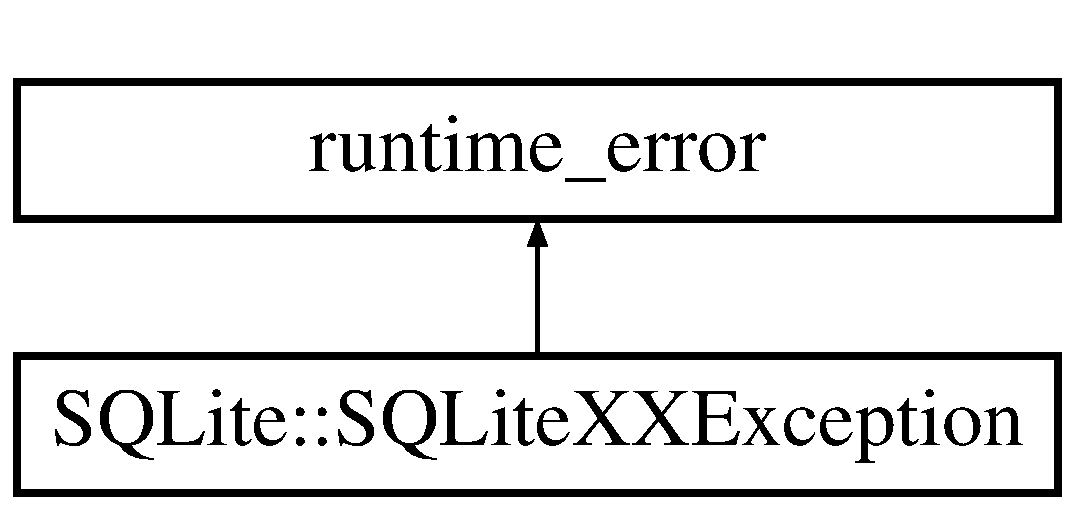
\includegraphics[height=2.000000cm]{class_s_q_lite_1_1_s_q_lite_x_x_exception}
\end{center}
\end{figure}
\subsection*{Public Member Functions}
\begin{DoxyCompactItemize}
\item 
\hypertarget{class_s_q_lite_1_1_s_q_lite_x_x_exception_ae0075cd411707f313b1832235f6d10dd}{{\bfseries S\-Q\-Lite\-X\-X\-Exception} (const std\-::string \&message)}\label{class_s_q_lite_1_1_s_q_lite_x_x_exception_ae0075cd411707f313b1832235f6d10dd}

\end{DoxyCompactItemize}


The documentation for this class was generated from the following file\-:\begin{DoxyCompactItemize}
\item 
src/Exception.\-h\end{DoxyCompactItemize}

\hypertarget{class_s_q_lite_1_1_statement}{\section{S\-Q\-Lite\-:\-:Statement Class Reference}
\label{class_s_q_lite_1_1_statement}\index{S\-Q\-Lite\-::\-Statement@{S\-Q\-Lite\-::\-Statement}}
}


Represents a single S\-Q\-L statement that has been compiled into binary form and is ready to be evaluated, aka \char`\"{}sqlite3\-\_\-stmt\char`\"{}.  




{\ttfamily \#include $<$Statement.\-h$>$}

Inheritance diagram for S\-Q\-Lite\-:\-:Statement\-:\begin{figure}[H]
\begin{center}
\leavevmode
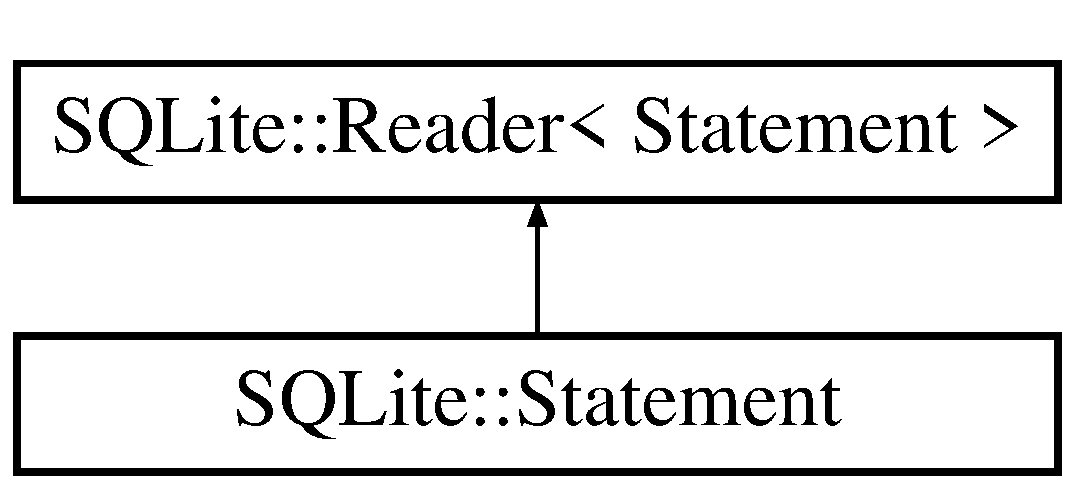
\includegraphics[height=2.000000cm]{class_s_q_lite_1_1_statement}
\end{center}
\end{figure}
\subsection*{Public Member Functions}
\begin{DoxyCompactItemize}
\item 
\hypertarget{class_s_q_lite_1_1_statement_ac4f1af971f094f30c445bcc18ffc4e27}{{\footnotesize template$<$typename... Values$>$ }\\{\bfseries Statement} (const \hyperlink{class_s_q_lite_1_1_d_b_connection}{D\-B\-Connection} \&connection, const std\-::string \&text, Values \&\&...values)}\label{class_s_q_lite_1_1_statement_ac4f1af971f094f30c445bcc18ffc4e27}

\item 
\hypertarget{class_s_q_lite_1_1_statement_a3857ee340dd2769fafe10259cf4858a3}{{\footnotesize template$<$typename... Values$>$ }\\{\bfseries Statement} (const \hyperlink{class_s_q_lite_1_1_d_b_connection}{D\-B\-Connection} \&connection, const std\-::u16string \&text, Values \&\&...values)}\label{class_s_q_lite_1_1_statement_a3857ee340dd2769fafe10259cf4858a3}

\item 
\hypertarget{class_s_q_lite_1_1_statement_a3b7793f1490a321159690cf096ec74d6}{{\bfseries operator bool} () const noexcept}\label{class_s_q_lite_1_1_statement_a3b7793f1490a321159690cf096ec74d6}

\item 
\hypertarget{class_s_q_lite_1_1_statement_a9052c143879aca6cf253925336464a8b}{sqlite3\-\_\-stmt $\ast$ \hyperlink{class_s_q_lite_1_1_statement_a9052c143879aca6cf253925336464a8b}{get\-Handle} () const noexcept}\label{class_s_q_lite_1_1_statement_a9052c143879aca6cf253925336464a8b}

\begin{DoxyCompactList}\small\item\em Returns pointer to the underlying \char`\"{}sqlite3\-\_\-stmt\char`\"{} object. \end{DoxyCompactList}\item 
{\footnotesize template$<$typename... Values$>$ }\\void \hyperlink{class_s_q_lite_1_1_statement_a1ecd8e2636b542314521eb68fbf1000e}{prepare} (\hyperlink{class_s_q_lite_1_1_d_b_connection}{D\-B\-Connection} const \&connection, const std\-::string \&text, Values \&\&...values)
\begin{DoxyCompactList}\small\item\em Turn an S\-Q\-L query into byte code. \end{DoxyCompactList}\item 
{\footnotesize template$<$typename... Values$>$ }\\void \hyperlink{class_s_q_lite_1_1_statement_a0d422eadca4b2e3f2e1b6e13af69f3cc}{prepare} (const \hyperlink{class_s_q_lite_1_1_d_b_connection}{D\-B\-Connection} \&connection, const std\-::u16string \&text, Values \&\&...values)
\begin{DoxyCompactList}\small\item\em Turn an S\-Q\-L query into byte code. \end{DoxyCompactList}\item 
bool \hyperlink{class_s_q_lite_1_1_statement_a6251d1119e978d1366113b4aa30899ef}{step} () const 
\begin{DoxyCompactList}\small\item\em Evaluates a prepared statement. \end{DoxyCompactList}\item 
\hypertarget{class_s_q_lite_1_1_statement_a9b489a2dc2707543eba55ce1e5d3682c}{int {\bfseries execute} () const }\label{class_s_q_lite_1_1_statement_a9b489a2dc2707543eba55ce1e5d3682c}

\item 
void \hyperlink{class_s_q_lite_1_1_statement_a0d4999fce90145852287c18c0d218ac6}{bind} (const int index, const int value) const 
\begin{DoxyCompactList}\small\item\em Binds an integer value to a parameters in an S\-Q\-L prepared statement. \end{DoxyCompactList}\item 
\hypertarget{class_s_q_lite_1_1_statement_ace8156c735b1e630e82a3840910e02cf}{void {\bfseries bind} (const int index, const double value) const }\label{class_s_q_lite_1_1_statement_ace8156c735b1e630e82a3840910e02cf}

\item 
\hypertarget{class_s_q_lite_1_1_statement_aab00e4b2d9a0d85ccaf2b058d0cc9523}{void {\bfseries bind} (const int index, const void $\ast$const value, const int size, Bind\-Type type=Bind\-Type\-::\-Transient) const }\label{class_s_q_lite_1_1_statement_aab00e4b2d9a0d85ccaf2b058d0cc9523}

\item 
\hypertarget{class_s_q_lite_1_1_statement_afc5e0d9485bfedc71e9863cdb3c3d11a}{void {\bfseries bind} (const int index, const \hyperlink{class_s_q_lite_1_1_blob}{Blob} \&value) const }\label{class_s_q_lite_1_1_statement_afc5e0d9485bfedc71e9863cdb3c3d11a}

\item 
\hypertarget{class_s_q_lite_1_1_statement_a3ed628586d99205a1443790e7dc1e36f}{void {\bfseries bind} (const int index, const char $\ast$const value, const int size=-\/1, Bind\-Type type=Bind\-Type\-::\-Transient) const }\label{class_s_q_lite_1_1_statement_a3ed628586d99205a1443790e7dc1e36f}

\item 
\hypertarget{class_s_q_lite_1_1_statement_a6b983503e072b56f2255b140dd271381}{void {\bfseries bind} (const int index, const char16\-\_\-t $\ast$const value, const int size=-\/1, Bind\-Type type=Bind\-Type\-::\-Transient) const }\label{class_s_q_lite_1_1_statement_a6b983503e072b56f2255b140dd271381}

\item 
\hypertarget{class_s_q_lite_1_1_statement_a2e33406ed4170291b9e3da490383a224}{void {\bfseries bind} (const int index, const std\-::string \&value) const }\label{class_s_q_lite_1_1_statement_a2e33406ed4170291b9e3da490383a224}

\item 
\hypertarget{class_s_q_lite_1_1_statement_a0a2d97dc865a1ebefb58f982fe5689a0}{void {\bfseries bind} (const int index, const std\-::u16string \&value) const }\label{class_s_q_lite_1_1_statement_a0a2d97dc865a1ebefb58f982fe5689a0}

\item 
\hypertarget{class_s_q_lite_1_1_statement_aa78aca5ae5830111b4097de1596c5eb0}{void {\bfseries bind} (const int index, std\-::string \&\&value) const }\label{class_s_q_lite_1_1_statement_aa78aca5ae5830111b4097de1596c5eb0}

\item 
\hypertarget{class_s_q_lite_1_1_statement_a0bf4a9fe041c5a95c099d8fd1e085ecd}{void {\bfseries bind} (const int index, std\-::u16string \&\&value) const }\label{class_s_q_lite_1_1_statement_a0bf4a9fe041c5a95c099d8fd1e085ecd}

\item 
\hypertarget{class_s_q_lite_1_1_statement_a30d8dec0baa340a358ce65a49ace23d8}{{\footnotesize template$<$typename T $>$ }\\void {\bfseries bind\-By\-Name} (const std\-::string \&name, T \&\&value)}\label{class_s_q_lite_1_1_statement_a30d8dec0baa340a358ce65a49ace23d8}

\item 
\hypertarget{class_s_q_lite_1_1_statement_a9b04cc93fd0242ea34d3e9e3a9cd88d3}{{\footnotesize template$<$typename... Values$>$ }\\void {\bfseries bind\-All} (Values \&\&...values) const }\label{class_s_q_lite_1_1_statement_a9b04cc93fd0242ea34d3e9e3a9cd88d3}

\item 
\hypertarget{class_s_q_lite_1_1_statement_a23bb702d61e121bfbb7adca6dc11acfb}{{\footnotesize template$<$typename... Values$>$ }\\void {\bfseries reset} (Values \&\&...values) const }\label{class_s_q_lite_1_1_statement_a23bb702d61e121bfbb7adca6dc11acfb}

\end{DoxyCompactItemize}


\subsection{Detailed Description}
Represents a single S\-Q\-L statement that has been compiled into binary form and is ready to be evaluated, aka \char`\"{}sqlite3\-\_\-stmt\char`\"{}. 

\subsection{Member Function Documentation}
\hypertarget{class_s_q_lite_1_1_statement_a0d4999fce90145852287c18c0d218ac6}{\index{S\-Q\-Lite\-::\-Statement@{S\-Q\-Lite\-::\-Statement}!bind@{bind}}
\index{bind@{bind}!SQLite::Statement@{S\-Q\-Lite\-::\-Statement}}
\subsubsection[{bind}]{\setlength{\rightskip}{0pt plus 5cm}void S\-Q\-Lite\-::\-Statement\-::bind (
\begin{DoxyParamCaption}
\item[{const int}]{index, }
\item[{const int}]{value}
\end{DoxyParamCaption}
) const}}\label{class_s_q_lite_1_1_statement_a0d4999fce90145852287c18c0d218ac6}


Binds an integer value to a parameters in an S\-Q\-L prepared statement. 


\begin{DoxyParams}{Parameters}
{\em index} & of the S\-Q\-L parameter to be set \\
\hline
{\em The} & integer value to bind to the parameter. \\
\hline
\end{DoxyParams}
\hypertarget{class_s_q_lite_1_1_statement_a1ecd8e2636b542314521eb68fbf1000e}{\index{S\-Q\-Lite\-::\-Statement@{S\-Q\-Lite\-::\-Statement}!prepare@{prepare}}
\index{prepare@{prepare}!SQLite::Statement@{S\-Q\-Lite\-::\-Statement}}
\subsubsection[{prepare}]{\setlength{\rightskip}{0pt plus 5cm}template$<$typename... Values$>$ void S\-Q\-Lite\-::\-Statement\-::prepare (
\begin{DoxyParamCaption}
\item[{{\bf D\-B\-Connection} const \&}]{connection, }
\item[{const std\-::string \&}]{text, }
\item[{Values \&\&...}]{values}
\end{DoxyParamCaption}
)\hspace{0.3cm}{\ttfamily [inline]}}}\label{class_s_q_lite_1_1_statement_a1ecd8e2636b542314521eb68fbf1000e}


Turn an S\-Q\-L query into byte code. 


\begin{DoxyParams}{Parameters}
{\em connection} & a successfully opened database connection \\
\hline
{\em text} & the statement to be compiled, encoded as U\-T\-F-\/8 \\
\hline
{\em values} & possible bindings \\
\hline
\end{DoxyParams}
\hypertarget{class_s_q_lite_1_1_statement_a0d422eadca4b2e3f2e1b6e13af69f3cc}{\index{S\-Q\-Lite\-::\-Statement@{S\-Q\-Lite\-::\-Statement}!prepare@{prepare}}
\index{prepare@{prepare}!SQLite::Statement@{S\-Q\-Lite\-::\-Statement}}
\subsubsection[{prepare}]{\setlength{\rightskip}{0pt plus 5cm}template$<$typename... Values$>$ void S\-Q\-Lite\-::\-Statement\-::prepare (
\begin{DoxyParamCaption}
\item[{const {\bf D\-B\-Connection} \&}]{connection, }
\item[{const std\-::u16string \&}]{text, }
\item[{Values \&\&...}]{values}
\end{DoxyParamCaption}
)\hspace{0.3cm}{\ttfamily [inline]}}}\label{class_s_q_lite_1_1_statement_a0d422eadca4b2e3f2e1b6e13af69f3cc}


Turn an S\-Q\-L query into byte code. 


\begin{DoxyParams}{Parameters}
{\em connection} & a successfully opened database connection \\
\hline
{\em text} & the statement to be compiled, encoded as U\-T\-F-\/16 \\
\hline
{\em values} & possible bindings \\
\hline
\end{DoxyParams}
\hypertarget{class_s_q_lite_1_1_statement_a6251d1119e978d1366113b4aa30899ef}{\index{S\-Q\-Lite\-::\-Statement@{S\-Q\-Lite\-::\-Statement}!step@{step}}
\index{step@{step}!SQLite::Statement@{S\-Q\-Lite\-::\-Statement}}
\subsubsection[{step}]{\setlength{\rightskip}{0pt plus 5cm}bool S\-Q\-Lite\-::\-Statement\-::step (
\begin{DoxyParamCaption}
{}
\end{DoxyParamCaption}
) const}}\label{class_s_q_lite_1_1_statement_a6251d1119e978d1366113b4aa30899ef}


Evaluates a prepared statement. 

This method can be called one or more times to evaluate the statement. \begin{DoxyReturn}{Returns}
true when there are more rows to iterate through and false when there are no more 
\end{DoxyReturn}

\begin{DoxyExceptions}{Exceptions}
{\em \hyperlink{class_s_q_lite_1_1_exception}{S\-Q\-Lite\-::\-Exception}} & or a derived class \\
\hline
\end{DoxyExceptions}


The documentation for this class was generated from the following files\-:\begin{DoxyCompactItemize}
\item 
src/Statement.\-h\item 
src/Statement.\-cpp\end{DoxyCompactItemize}

\hypertarget{class_s_q_lite_1_1_transaction}{\section{S\-Q\-Lite\-:\-:Transaction Class Reference}
\label{class_s_q_lite_1_1_transaction}\index{S\-Q\-Lite\-::\-Transaction@{S\-Q\-Lite\-::\-Transaction}}
}


R\-A\-I\-I encapsulation of the S\-Q\-Lite Transactions.  




{\ttfamily \#include $<$Transaction.\-h$>$}

Inheritance diagram for S\-Q\-Lite\-:\-:Transaction\-:\begin{figure}[H]
\begin{center}
\leavevmode
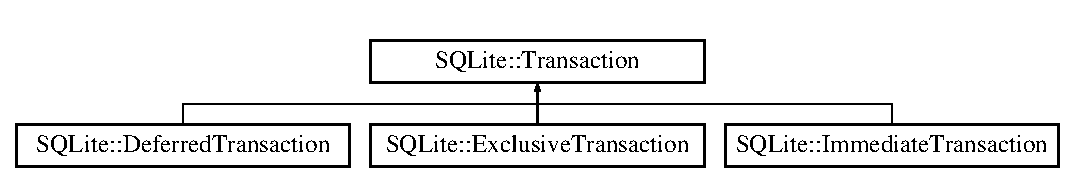
\includegraphics[height=2.000000cm]{class_s_q_lite_1_1_transaction}
\end{center}
\end{figure}
\subsection*{Public Member Functions}
\begin{DoxyCompactItemize}
\item 
\hyperlink{class_s_q_lite_1_1_transaction_a27add1a1db2dd8cd5935c78a63ad556b}{Transaction} (\hyperlink{class_s_q_lite_1_1_d_b_connection}{D\-B\-Connection} \&connection, const Transaction\-Type type)
\begin{DoxyCompactList}\small\item\em Begins the S\-Q\-Lite transaction. \end{DoxyCompactList}\item 
\hypertarget{class_s_q_lite_1_1_transaction_a43c5e67a10b9698b7f6dad73539feb94}{virtual \hyperlink{class_s_q_lite_1_1_transaction_a43c5e67a10b9698b7f6dad73539feb94}{$\sim$\-Transaction} () noexcept}\label{class_s_q_lite_1_1_transaction_a43c5e67a10b9698b7f6dad73539feb94}

\begin{DoxyCompactList}\small\item\em Safely rollback the transaction if it has not been commited. \end{DoxyCompactList}\item 
\hypertarget{class_s_q_lite_1_1_transaction_a9b251d84198cdc2c0208ad566fec0287}{virtual void \hyperlink{class_s_q_lite_1_1_transaction_a9b251d84198cdc2c0208ad566fec0287}{commit} ()}\label{class_s_q_lite_1_1_transaction_a9b251d84198cdc2c0208ad566fec0287}

\begin{DoxyCompactList}\small\item\em Commit the transaction. \end{DoxyCompactList}\end{DoxyCompactItemize}
\subsection*{Public Attributes}
\begin{DoxyCompactItemize}
\item 
\hypertarget{class_s_q_lite_1_1_transaction_ac83d867e6fd7ec9dfe30b3c32bbcfee0}{const Transaction\-Type {\bfseries type}}\label{class_s_q_lite_1_1_transaction_ac83d867e6fd7ec9dfe30b3c32bbcfee0}

\end{DoxyCompactItemize}


\subsection{Detailed Description}
R\-A\-I\-I encapsulation of the S\-Q\-Lite Transactions. 

\subsection{Constructor \& Destructor Documentation}
\hypertarget{class_s_q_lite_1_1_transaction_a27add1a1db2dd8cd5935c78a63ad556b}{\index{S\-Q\-Lite\-::\-Transaction@{S\-Q\-Lite\-::\-Transaction}!Transaction@{Transaction}}
\index{Transaction@{Transaction}!SQLite::Transaction@{S\-Q\-Lite\-::\-Transaction}}
\subsubsection[{Transaction}]{\setlength{\rightskip}{0pt plus 5cm}S\-Q\-Lite\-::\-Transaction\-::\-Transaction (
\begin{DoxyParamCaption}
\item[{{\bf D\-B\-Connection} \&}]{connection, }
\item[{const Transaction\-Type}]{type}
\end{DoxyParamCaption}
)}}\label{class_s_q_lite_1_1_transaction_a27add1a1db2dd8cd5935c78a63ad556b}


Begins the S\-Q\-Lite transaction. 


\begin{DoxyParams}[1]{Parameters}
\mbox{\tt in}  & {\em connection} & the database connection to begin the transaction on \\
\hline
\end{DoxyParams}


The documentation for this class was generated from the following files\-:\begin{DoxyCompactItemize}
\item 
src/Transaction.\-h\item 
src/Transaction.\-cpp\end{DoxyCompactItemize}

\hypertarget{class_s_q_lite_1_1_value}{\section{S\-Q\-Lite\-:\-:Value Class Reference}
\label{class_s_q_lite_1_1_value}\index{S\-Q\-Lite\-::\-Value@{S\-Q\-Lite\-::\-Value}}
}


A S\-Q\-Lite dynamically typed value object, aka \char`\"{}sqlite3\-\_\-value\char`\"{}.  




{\ttfamily \#include $<$Value.\-h$>$}

\subsection*{Public Member Functions}
\begin{DoxyCompactItemize}
\item 
\hypertarget{class_s_q_lite_1_1_value_ace0be7092c23d5e3f4312db057d86997}{{\bfseries Value} (const sqlite3\-\_\-value $\ast$const value)}\label{class_s_q_lite_1_1_value_ace0be7092c23d5e3f4312db057d86997}

\item 
\hypertarget{class_s_q_lite_1_1_value_acd6e10f2a509c8a0be20237d4b3a0fc7}{{\bfseries Value} (const \hyperlink{class_s_q_lite_1_1_value}{Value} \&other)}\label{class_s_q_lite_1_1_value_acd6e10f2a509c8a0be20237d4b3a0fc7}

\item 
\hypertarget{class_s_q_lite_1_1_value_a531d4f514b9abe1eb1f47a277737b953}{{\bfseries Value} (\hyperlink{class_s_q_lite_1_1_value}{Value} \&\&other)}\label{class_s_q_lite_1_1_value_a531d4f514b9abe1eb1f47a277737b953}

\item 
\hypertarget{class_s_q_lite_1_1_value_a879c07032f32606d277a8f6581a13abf}{\hyperlink{class_s_q_lite_1_1_value}{Value} \& {\bfseries operator=} (const \hyperlink{class_s_q_lite_1_1_value}{Value} \&other)}\label{class_s_q_lite_1_1_value_a879c07032f32606d277a8f6581a13abf}

\item 
\hypertarget{class_s_q_lite_1_1_value_ab80d7cf9eb8a462b23459d0fbba80277}{\hyperlink{class_s_q_lite_1_1_value}{Value} \& {\bfseries operator=} (\hyperlink{class_s_q_lite_1_1_value}{Value} \&\&other)}\label{class_s_q_lite_1_1_value_ab80d7cf9eb8a462b23459d0fbba80277}

\item 
\hypertarget{class_s_q_lite_1_1_value_adc0c8d347cbd6dbbd38c85ff755c9100}{sqlite3\-\_\-value $\ast$ \hyperlink{class_s_q_lite_1_1_value_adc0c8d347cbd6dbbd38c85ff755c9100}{get\-Handle} () const noexcept}\label{class_s_q_lite_1_1_value_adc0c8d347cbd6dbbd38c85ff755c9100}

\begin{DoxyCompactList}\small\item\em Returns pointer to the underlying \char`\"{}sqlite3\-\_\-value\char`\"{} object. \end{DoxyCompactList}\item 
\hypertarget{class_s_q_lite_1_1_value_a7dc198b9bcd56e1a00b4277d67e2fe94}{int {\bfseries get\-Int} () const noexcept}\label{class_s_q_lite_1_1_value_a7dc198b9bcd56e1a00b4277d67e2fe94}

\item 
\hypertarget{class_s_q_lite_1_1_value_afea7de5c78253675c70f1d4c49740e37}{int64\-\_\-t {\bfseries get\-Int64} () const noexcept}\label{class_s_q_lite_1_1_value_afea7de5c78253675c70f1d4c49740e37}

\item 
\hypertarget{class_s_q_lite_1_1_value_a196e4e06082b963730d766f99ccb3917}{unsigned int {\bfseries get\-U\-Int} () const noexcept}\label{class_s_q_lite_1_1_value_a196e4e06082b963730d766f99ccb3917}

\item 
\hypertarget{class_s_q_lite_1_1_value_a7976bd8973e60229f32d57d80b309eef}{double {\bfseries get\-Double} () const noexcept}\label{class_s_q_lite_1_1_value_a7976bd8973e60229f32d57d80b309eef}

\item 
\hypertarget{class_s_q_lite_1_1_value_a271c3d7f1de010f03197f5c72fd60d61}{const \hyperlink{class_s_q_lite_1_1_blob}{Blob} {\bfseries get\-Blob} () const noexcept}\label{class_s_q_lite_1_1_value_a271c3d7f1de010f03197f5c72fd60d61}

\item 
\hypertarget{class_s_q_lite_1_1_value_ae31b8ba26dec2668d11a49ad895e2267}{const std\-::string {\bfseries get\-String} () const noexcept}\label{class_s_q_lite_1_1_value_ae31b8ba26dec2668d11a49ad895e2267}

\item 
\hypertarget{class_s_q_lite_1_1_value_a693c71ee6c918f92e4378e91318a7694}{const std\-::u16string {\bfseries get\-U16\-String} () const noexcept}\label{class_s_q_lite_1_1_value_a693c71ee6c918f92e4378e91318a7694}

\item 
\hypertarget{class_s_q_lite_1_1_value_a03a193504f0c5fd751302a6ec8d01845}{int {\bfseries get\-Bytes} () const noexcept}\label{class_s_q_lite_1_1_value_a03a193504f0c5fd751302a6ec8d01845}

\item 
\hypertarget{class_s_q_lite_1_1_value_ac43f7a22f87464aceaef9855e9700ff7}{Type {\bfseries get\-Type} () const noexcept}\label{class_s_q_lite_1_1_value_ac43f7a22f87464aceaef9855e9700ff7}

\item 
\hypertarget{class_s_q_lite_1_1_value_adbb8614964a6724dd5ec65dcdb0d4ab1}{{\bfseries operator int} () const }\label{class_s_q_lite_1_1_value_adbb8614964a6724dd5ec65dcdb0d4ab1}

\item 
\hypertarget{class_s_q_lite_1_1_value_a9a10fa6ba990f034a511764fc7e3b7f9}{{\bfseries operator unsigned int} () const }\label{class_s_q_lite_1_1_value_a9a10fa6ba990f034a511764fc7e3b7f9}

\item 
\hypertarget{class_s_q_lite_1_1_value_a0aa282facbe60435956643ad4f01e413}{{\bfseries operator unsigned long} () const }\label{class_s_q_lite_1_1_value_a0aa282facbe60435956643ad4f01e413}

\item 
\hypertarget{class_s_q_lite_1_1_value_a1f36acd2099170093c5285b04524ca76}{{\bfseries operator long} () const }\label{class_s_q_lite_1_1_value_a1f36acd2099170093c5285b04524ca76}

\item 
\hypertarget{class_s_q_lite_1_1_value_ab5ecb2b66ce289a0023961e6c2959926}{{\bfseries operator long long} () const }\label{class_s_q_lite_1_1_value_ab5ecb2b66ce289a0023961e6c2959926}

\item 
\hypertarget{class_s_q_lite_1_1_value_a44e0812e9ede7042f1d3497fbafd4b15}{{\bfseries operator double} () const }\label{class_s_q_lite_1_1_value_a44e0812e9ede7042f1d3497fbafd4b15}

\item 
\hypertarget{class_s_q_lite_1_1_value_a3481e1de221db430e8efe10d572ff3ba}{{\bfseries operator const Blob} () const }\label{class_s_q_lite_1_1_value_a3481e1de221db430e8efe10d572ff3ba}

\item 
\hypertarget{class_s_q_lite_1_1_value_a39582758e6f28c6bc626e3e5e4cc90e1}{{\bfseries operator const std\-::string} () const }\label{class_s_q_lite_1_1_value_a39582758e6f28c6bc626e3e5e4cc90e1}

\item 
\hypertarget{class_s_q_lite_1_1_value_a7313e05100aa0982b81dcc006dc8b5d5}{{\bfseries operator const std\-::u16string} () const }\label{class_s_q_lite_1_1_value_a7313e05100aa0982b81dcc006dc8b5d5}

\end{DoxyCompactItemize}


\subsection{Detailed Description}
A S\-Q\-Lite dynamically typed value object, aka \char`\"{}sqlite3\-\_\-value\char`\"{}. 

\hyperlink{class_s_q_lite_1_1_value}{Value} objects represent all values that can be stored in a database table. A \hyperlink{class_s_q_lite_1_1_value}{Value} object may be either \char`\"{}protected\char`\"{} or \char`\"{}unprotected\char`\"{} which refers to whether or not a mutex is held. An internal mutex is held for a protected value object but not for an unprotected one. If S\-Q\-Lite is compiled to be single-\/threaded or if S\-Q\-Lite is run in one of reduced mutex modes then there is no distinction between protected and unprotected sqlite3\-\_\-value objects. A \hyperlink{class_s_q_lite_1_1_value}{Value} objects will always be \char`\"{}protected\char`\"{} as it stores a sqlite3\-\_\-value objects created from calling the sqlite3\-\_\-value\-\_\-dup() interface which produces a \char`\"{}protected\char`\"{} \char`\"{}sqlite3\-\_\-value\char`\"{} from an \char`\"{}unprotected\char`\"{} one. Only use a \hyperlink{class_s_q_lite_1_1_value}{Value} object in the same thread as the S\-Q\-L function that created it. 

The documentation for this class was generated from the following files\-:\begin{DoxyCompactItemize}
\item 
src/Value.\-h\item 
src/Value.\-cpp\end{DoxyCompactItemize}

%--- End generated contents ---

% Index
\newpage
\phantomsection
\addcontentsline{toc}{chapter}{Index}
\printindex

\end{document}
